\documentclass[12pt,oneside,titlepage]{scrartcl} 

\newcommand{\myAutor}{Rico  (Matrikelnummer 12345)\\ \> \> \> 
Henning   (Matrikelnummer 12345)\\ \> \> \> 
Julian  (Matrikelnummer 12345)} % Autor
\newcommand{\myAdresse}{Stra\ss e 123 \\ \> \> \> 57xxx Siegerland} % Adresse
\newcommand{\myTitel}{Browser RPG-Adventure} % Titel der Arbeit
\newcommand{\myBetreuer}{Daniel Bitzer} % Betreuer
\newcommand{\myLehrveranstaltung}{Web Technologie} % Lehrveranstaltung
\newcommand{\myMatrikelNr}{123456} % Matrikelnummer
\newcommand{\myOrt}{Siegen} % Ort
\newcommand{\myAbgabeDatum}{\today} % Datum der Abgabe
\newcommand{\mySemesterZahl}{5} % Semesterzahl
\newcommand{\myHochschulName}{FOM Hochschule für Oekonomie \& Management Essen} % Name der Hochschule
\newcommand{\myHochschulStandort}{Siegen} % Standort der Hochschule
\newcommand{\myStudiengang}{Wirtschaftsinformatik} % Studiengang
\newcommand{\myThesisArt}{Seminararbeit als Projektdokumentation} % Art der Arbeit
\newcommand{\myAkademischerGrad}{Bachelor of Science (B. Sc.)} % Zu erlangender akademische Grad
\newcommand{\myFirma}{Mustermann GmbH} % Firma

\usepackage[ngerman]{babel}
\selectlanguage{ngerman}
\usepackage[babel,german=quotes]{csquotes}

\usepackage[utf8]{luainputenc}
\usepackage[T1]{fontenc}
\usepackage{fancyhdr}
\usepackage{fancybox}
\usepackage[a4paper, left=4cm, right=2cm, top=4cm, bottom=2cm]{geometry}
\usepackage{graphicx}
\usepackage{colortbl}
\usepackage[capposition=top]{floatrow}
\usepackage{array}
\usepackage{float}      %Positionierung von Abb. und Tabellen mit [H] erzwingen
\usepackage{footnote}
\usepackage[singlelinecheck=false, labelfont=bf, font=bf]{caption} % Tabellendesign lt. Leitfaden
\usepackage{caption}
\usepackage{enumitem}
\usepackage{amssymb}
\usepackage{mathptmx}
\usepackage[scaled=0.9]{helvet} 
\usepackage{courier}
\usepackage{amsmath}
\usepackage[table]{xcolor}
\usepackage{marvosym}			% Verwendung von Symbolen, z.B. perfektes Eurozeichen
\usepackage[colorlinks=true,linkcolor=black]{hyperref}
\definecolor{darkblack}{rgb}{0,0,0}
\hypersetup{colorlinks=true, breaklinks=true, linkcolor=darkblack, menucolor=darkblack, urlcolor=darkblack}
\renewcommand\familydefault{\sfdefault}
\usepackage{ragged2e}

\usepackage[hang, multiple]{footmisc} % Mehrere Fussnoten nacheinander mit Komma separiert
\setlength{\footnotemargin}{1em}

%\usepackage{todonotes} % todo Aufgaben als Kommentare verfassen für verschiedene Editoren

\usepackage{epstopdf} %Pakete für Tabellen
\usepackage{nicefrac} % Brüche
\usepackage{multirow}
\usepackage{rotating} % vertikal schreiben
\usepackage{mdwlist}
\usepackage{tabularx}% für breitenangabe

\definecolor{dunkelgrau}{rgb}{0.8,0.8,0.8}
\definecolor{hellgrau}{rgb}{0.0,0.7,0.99}
% Colors for listings
\definecolor{mauve}{rgb}{0.58,0,0.82}
\definecolor{dkgreen}{rgb}{0,0.6,0}

\usepackage{listings} % sauber formatierter Quelltext
% JavaScript als Sprache definieren:
\lstdefinelanguage{JavaScript}{
	keywords={break, super, case, extends, switch, catch, finally, for, const, function, try, continue, if, typeof, debugger, var, default, in, void, delete, instanceof, while, do, new, with, else, return, yield, enum, let, await},
	keywordstyle=\color{blue}\bfseries,
	ndkeywords={class, export, boolean, throw, implements, import, this, interface, package, private, protected, public, static},
	ndkeywordstyle=\color{darkgray}\bfseries,
	identifierstyle=\color{black},
	sensitive=false,
	comment=[l]{//},
	morecomment=[s]{/*}{*/},
	commentstyle=\color{purple}\ttfamily,
	stringstyle=\color{red}\ttfamily,
	morestring=[b]',
	morestring=[b]"
}

\lstset{
	%language=JavaScript,
	numbers=left,
	numberstyle=\tiny,
	numbersep=5pt,
	breaklines=true,
	showstringspaces=false,
	frame=l ,
	xleftmargin=5pt,
	xrightmargin=5pt,
	basicstyle=\ttfamily\scriptsize, 
	stepnumber=1,
	keywordstyle=\color{blue},          % keyword style
  	commentstyle=\color{dkgreen},       % comment style
  	stringstyle=\color{mauve}         % string literal style
}

\usepackage[
    style           = apa6, 
    uniquelist      = false,    
    maxcitenames    = 6,
    backend         = biber,
	urldate         = short,
	uniquename 		= true,
	language		= ngerman
	]{biblatex} 
		
	%% START Block für Funktion (1. Nennung von 2-6 Autoren: Alle Namen, danach nur noch 1. Name + et.al) 
	\usepackage{lmodern} 
	\makeatletter
	\newcommand{\apamaxcitenames}{6}
	\DeclareNameFormat{labelname}{%
	  \ifthenelse{\value{uniquelist}>1}
		{\numdef\cbx@min{\value{uniquelist}}}
		{\numdef\cbx@min{\value{minnames}}}%
	  \ifboolexpr{test {\ifnumcomp{\value{listcount}}{=}{1}}
				  or test {\ifnumcomp{\value{listtotal}}{=}{2}}}
		{\usebibmacro{labelname:doname}%
		  {\namepartfamily}%
		  {\namepartfamilyi}%
		  {\namepartgiven}%
		  {\namepartgiveni}%
		  {\namepartprefix}%
		  {\namepartprefixi}%
		  {\namepartsuffix}%
		  {\namepartsuffixi}}
		{\ifboolexpr{test {\ifnumcomp{\value{listtotal}}{>}{\apamaxcitenames}}
					 or test {\ifciteseen}}
		 {\ifnumcomp{\value{listcount}}{<}{\cbx@min + 1}
		   {\usebibmacro{labelname:doname}%
			 {\namepartfamily}%
			 {\namepartfamilyi}%
			 {\namepartgiven}%
			 {\namepartgiveni}%
			 {\namepartprefix}%
			 {\namepartprefixi}%
			 {\namepartsuffix}%
			 {\namepartsuffixi}}
		   {}%
		  \ifnumcomp{\value{listcount}}{=}{\cbx@min + 1}
			{\ifnumcomp{\value{listcount}}{<}{\value{listtotal}}
			  {\printdelim{andothersdelim}\bibstring{andothers}}
			  {\usebibmacro{labelname:doname}%
				{\namepartfamily}%
				{\namepartfamilyi}%
				{\namepartgiven}%
				{\namepartgiveni}%
				{\namepartprefix}%
				{\namepartprefixi}%
				{\namepartsuffix}%
				{\namepartsuffixi}}}
			{}%
		  \ifnumcomp{\value{listcount}}{>}{\cbx@min + 1}
		   {\relax}%
		   {}}%
		 {\usebibmacro{labelname:doname}%
		   {\namepartfamily}%
		   {\namepartfamilyi}%
		   {\namepartgiven}%
		   {\namepartgiveni}%
		   {\namepartprefix}%
		   {\namepartprefixi}%
		   {\namepartsuffix}%
		   {\namepartsuffixi}}}}
	\makeatother 
	\DeclareLanguageMapping{ngerman}{ngerman-apa}
	%% ENDE Block für Funktion (1. Nennung von 2-6 Autoren: Alle Namen, danach nur noch 1. Name + et.al)
	
	\DeclareDelimFormat*{finalnamedelim}{\addspace\bibstring{and}\space} % In Parencite von "&" auf "und" ändern
	\hypersetup{hidelinks}  %Grüne Links auf Literaturverz. unterdrücken.
	\setlength\bibitemsep{1.3ex} % Abstände im Literaturverzeichnis erhöhen
	\setlength\bibnamesep{1.0ex}
	\AtBeginBibliography{\singlespacing} % Zeilenabstand im Literaturverzeichnis ist Einzeilig - siehe Leitfaden S. 14
	\urlstyle{same} %Standard-Font für Link anstelle der "Schreibmaschinenschrift"
	\DeclareFieldFormat[misc]{urldate}{[#1\printfield{urldate}].} 	% Anpassung @online + @misc Bibl: Datum in eckigen Klammern ans Ende
	\DeclareFieldFormat[misc]{title}{\mkbibemph{#1}} %Anpassung @online + @misc Titel Kursiv	
	\DeclareFieldFormat[misc]{url}{Verfügbar unter\space \url{#1}} 	%Anpassung @online + @misc Text vor URL
	\renewbibmacro*{url+urldate}{\usebibmacro{url}\setunit{\addspace}\usebibmacro{urldate}}  % URL vor Abrufdatum setzen + getrennte Wörter "Verfügbar" und "Unter" entfernen
%%%% APA ENDE

\addbibresource{literatur.bib} %Bib-Datei einbinden
%\nocite{*} % Die folgende Zeile trägt ALLE Werke aus literatur.bib in das Verz. ein, auskommentieren um nur die anzuzeigen, die zitiert wurden


\usepackage{hyphsubst} %Silbentrennung
\HyphSubstIfExists{ngerman-x-latest}{%
\HyphSubstLet{ngerman}{ngerman-x-latest}}{}

\graphicspath{{./}{./media/}} % Pfad fuer Abbildungen

\usepackage{titletoc} % Weitere Ebene einfügen
\makeatletter

% Setze die Tiefe des Inhaltsverzeichnis auf 4 Ebenen -  Damit erscheinen \paragraph-Sektionen auch im Inhaltsverzeichnis
\setcounter{secnumdepth}{4}
\setcounter{tocdepth}{2}

% Fuege Abstand nach unten wie in einer normalen \section hinzu
\renewcommand{\paragraph}{%
  \@startsection{paragraph}{4}%
  {\z@}{3.25ex \@plus 1ex \@minus .2ex}{1.5ex plus 0.2ex}%
  {\normalfont\normalsize\bfseries\sffamily}%
}

\makeatother

\usepackage{appendix} % Paket für die Nutzung von Anhängen
\usepackage{setspace} % Zeilenabstand 1,5-zeilig
\onehalfspacing

\setlength{\parindent}{0mm} % Absätze durch eine neue Zeile
\setlength{\parskip}{0.8em plus 0.5em minus 0.3em}

\sloppy					%Abstände variieren
\pagestyle{headings}

\usepackage[printonlyused]{acronym} % Abkürzungsverzeichnis


% PDF Meta Daten setzen
\hypersetup{
    pdfinfo={
        Title={Browser RPG-Adventure},
        Subject={\myStudiengang},
        Author={\myAutor},
        Build=1.1
    }
}

% Umlaute in Code korrekt darstellen - siehe  https://en.wikibooks.org/wiki/LaTeX/Source_Code_Listings
\lstset{literate=
	{á}{{\'a}}1 {é}{{\'e}}1 {í}{{\'i}}1 {ó}{{\'o}}1 {ú}{{\'u}}1
	{Á}{{\'A}}1 {É}{{\'E}}1 {Í}{{\'I}}1 {Ó}{{\'O}}1 {Ú}{{\'U}}1
	{à}{{\`a}}1 {è}{{\`e}}1 {ì}{{\`i}}1 {ò}{{\`o}}1 {ù}{{\`u}}1
	{À}{{\`A}}1 {È}{{\'E}}1 {Ì}{{\`I}}1 {Ò}{{\`O}}1 {Ù}{{\`U}}1
	{ä}{{\"a}}1 {ë}{{\"e}}1 {ï}{{\"i}}1 {ö}{{\"o}}1 {ü}{{\"u}}1
	{Ä}{{\"A}}1 {Ë}{{\"E}}1 {Ï}{{\"I}}1 {Ö}{{\"O}}1 {Ü}{{\"U}}1
	{â}{{\^a}}1 {ê}{{\^e}}1 {î}{{\^i}}1 {ô}{{\^o}}1 {û}{{\^u}}1
	{Â}{{\^A}}1 {Ê}{{\^E}}1 {Î}{{\^I}}1 {Ô}{{\^O}}1 {Û}{{\^U}}1
	{œ}{{\oe}}1 {Œ}{{\OE}}1 {æ}{{\ae}}1 {Æ}{{\AE}}1 {ß}{{\ss}}1
	{ű}{{\H{u}}}1 {Ű}{{\H{U}}}1 {ő}{{\H{o}}}1 {Ő}{{\H{O}}}1
	{ç}{{\c c}}1 {Ç}{{\c C}}1 {ø}{{\o}}1 {å}{{\r a}}1 {Å}{{\r A}}1
	{€}{{\EUR}}1 {£}{{\pounds}}1 {„}{{\glqq{}}}1
}

\pagestyle{fancy} % Kopfbereich / Header definieren
\fancyhf{} % Seitenzahl oben, mittig, mit Strichen beidseits: \fancyhead[C]{-\ \thepage\ -}

\fancyhead[C]{\thepage} % Seitenzahl oben, mittig, entsprechend Leitfaden ohne Striche beidseits
\renewcommand{\headrulewidth}{0.4pt} % Waagerechte Linie unterhalb des Kopfbereiches anzeigen. Alternativ weg: \renewcommand{\headrulewidth}{0pt}

\begin{document} % Start the document here

\pagenumbering{Roman}								% Seitennumerierung auf römisch umstellen
\renewcommand{\refname}{Literaturverzeichnis}		% "Literatur" in "Literaturverzeichnis" umbenennen
\newcolumntype{C}{>{\centering\arraybackslash}X}	% Neuer Tabellen-Spalten-Typ: Zentriert und umbrechbar

\begin{titlepage} % Titlepage/Deckblatt
	\newgeometry{left=2cm, right=2cm, top=2cm, bottom=2cm}
	\begin{center}
		\textbf{\myHochschulName}\\
		\textbf{Hochschulzentrum \myHochschulStandort}\\
		\vspace{1.5cm}
			
\includegraphics[width=3cm]{media/fomLogo} \\
		\vspace{1.5cm}
		Berufsbegleitender Studiengang\\
		\myStudiengang, \mySemesterZahl. Semester\\
		\vspace{2cm}
		\textbf{\myThesisArt}\\
		%\textbf{zur Erlangung des Grades eines	}\\
		%\textbf{\myAkademischerGrad}\\
		% Oder für Hausarbeiten:
		\textbf{im Rahmen der Lehrveranstaltung}\\
		\textbf{\myLehrveranstaltung}\\
		\vspace{2cm}
		über das Thema\\
		\Large{\myTitel}\\
		\vspace{0.2cm}
	\end{center}
	\normalsize
	\vfill
	\begin{tabbing}
		Links \= Mitte \=Mittez \= Rechts\kill
		Betreuer: \> \> \>\myBetreuer\\
		\> \> \\
		Autoren: \> \> \> \myAutor\\
		%\> \> \>  Matrikelnummer: \myMatrikelNr\\
		%\> \> \> \myAdresse\\
		\> \> \>  \\
		Abgabe: \> \> \> \myAbgabeDatum
	\end{tabbing}
\end{titlepage}

%-------Ende Titelseite-------------


% Sperrvermerk
%\newpage
%\thispagestyle{empty}
%\section*{Sperrvermerk}
%Die vorliegende Abschlussarbeit mit dem Titel \enquote{\myTitel} enthält unternehmensinterne Daten der Firma \myFirma . Daher ist sie nur zur Vorlage bei der FOM sowie den Begutachtern der Arbeit bestimmt. Für die Öffentlichkeit und dritte Personen darf sie nicht zugänglich sein.
%\par\medskip
%\par\medskip
%\_\_\_\_\_\_\_\_\_\_\_\_\_\_\_\_\_\_\_\_\_\_\_\_ \hspace{1.5cm} \_\_\_\_\_\_\_\_\_\_\_\_\_\_\_\_\_\_\_\_\_\_\_\_ \\
%(Ort, Datum)\hspace{4.5cm}
%(Eigenhändige Unterschrift)
%\newpage

% 
% Inhaltsverzeichnis
\setcounter{page}{2}
\addtocontents{toc}{\protect\enlargethispage{-20mm}}
\clearpage
\tableofcontents
\newpage
\setcounter{tocdepth}{2} %wurde  in zusaetzlichesMaterial.tex auf 0 gesetzt um Inhalt des Anhangs zu verbergen. Dadurch gehen allerdings Abbildungs und Tabellenverzeichnis kaputt.

%\addcontentsline{toc}{section}{Abbildungsverzeichnis} % Falls das Abkürzungsverzeichnis im Inhaltsverzeichnis angezeigt werden 
%\section*{Abbildungsverzeichnis} % Abbildungsverzeichnis
\listoffigures % Abbildungsverzeichnis
\newpage

%\addcontentsline{toc}{section}{Tabellenverzeichnis} % Falls das Abkürzungsverzeichnis im Inhaltsverzeichnis angezeigt werden 
%\section*{Tabellenverzeichnis} % Tabellenverzeichnis
\listoftables % Tabellenverzeichnis
\newpage

%\addcontentsline{toc}{section}{Abkürzungsverzeichnis} % Falls das Abkürzungsverzeichnis im Inhaltsverzeichnis angezeigt werden soll einkommentieren.
\section*{Abkürzungsverzeichnis} % Abkürzungsverzeichnis

\begin{acronym}[WoWi]\itemsep0pt %der Parameter in Klammern sollte die längste Abkürzung sein. Damit wird der Abstand zwischen Abkürzung und Übersetzung festgelegt
	\acro{PoC}{Proof of Concept}
	\acro{WoWi}{Wohnungswirtschaft}
\end{acronym}
\newpage

\pagenumbering{arabic} % Seitennummerierung auf arabisch und ab 1 beginnend umstellen
\setcounter{page}{1}










%-----------------------------------
% Abschnite der Arbeit
%----------------------------



\section{Aufgabenbeschreibung}

(TODO!): Rico schreibt das.

Umfang 1-3 Seiten


\subsection{Was ist das Ziel der Projektarbeit? Worin bestehen die (wahrscheinlichen) Herausforderungen? (allg. technisch und auch persönlich)}

Primär: 
Fertiges, spielbares Programm 
Projektablauf erfolgreich gestalten 
Web-Technologien nutzen
Fokus auf die technische Umsetzung, Gameplay sekundär

Sekundär: 
Lernkurve
Projektmanagement leben
Erfahrungen im Spieldesign 

Herausforderungen (siehe \ref{2021-11-27-projektskizze-2})

\begin{itemize}
    \item techn. Umsetzbark.
    \item Zeit
    \item Know How
    \item Fokusverlust
    \item geeignete Aufgabefelder für eine Aufteilung finden 
\end{itemize}

Am Ende der Spieleentwiklung soll als primäres Ziel der Projektarbeit eine Art RPG (RolePlayingGame) mit Fantasysetting stehen, bei dem es zu aller erst um die Fertigstellung des kompletten Spielumfangs und nicht nur einiger Teilbereiche geht. Das Spiel soll also von Anfang bis Ende durchgespielt werden können und alle an das Projekt gefordertengestellten Anforderungen erfüllen und die gewünsten Inhalte bieten. Im Einzelnen sind im o. g. Zusammenhang folgende Dinge zu nennen. Das Spiel muss mit einem gängigem Browser online spielbar sein, es soll sowol Singelplayer- als auch Multiplayerelemente enthalten und es wird verschiedene Charakterklassen geben, die sich in ihren Fähigkeiten klar von einander unterscheiden. Im Laufe des Spiels werden sich, bei erreichen bestimmter Grenzen in einem für jeden Charackter eigenem Erfahrungspools, diese Fähigkeiten verbessen. Des weiteren wird es vom Projekteam unabhängig vom Endproduckt ebenfalls als primäres Ziel angesehen, den Projektablauf erfolgreich zu gestallten.
Als Sekundäre Ziele, also den primären Zielen klar untergeortnet, sieht die Projektgruppe die Spielerfahrung der einzelnen Spieler. Es ist allerdings angedacht diese im Ramen der Möglichkeiten so intensiv wie möglich zu gestallten, jedoch steht wie oben bereits erwähnt die Umsetzung der Vorgaben im Vordergrund. Außerdem möchte jeder der Teilnehmer an diesem Projekt Erfahrung im Spieldesign sammeln.
Die Herausforderungen in diesem Projekt sind recht vielfältig und sind grob in technisch und persönlich zu gliedern. Zu ersterem ist zu zählen, dass zu Beginn des Projekts nicht klar ist, ob das vom Team ersteinmal theoretisch entwickelte Konzept auch real, technisch umzusetzen ist. Zum einen weil nicht sicher ist ob die gewählte technische Plattform geeiget ist und zum anderen weil nicht klar ist ob das Know-how des Teams reicht um das gewollte in ein fertiges Endproduckt zu gießen. Außerdem könnten Rechte an Grafiken, Musik/Sounds und vielleicht sogar Programmcode zum Problem werden. Die Persönlichen herausforderungen liegen darin, das ganze Projekt zeilich so zu gestalten, dass es neben der hauptberuflichen Tätigkeit des Projektteams, noch genug Zeit für die Umsetzung bleibt. Und Krankheit oder Karantäne in der aktuellen Pandemie von einzelnen Teammitgliedern könnte den zeitlichen Ramen ebenfalls in Gefahr bringen. Auch muss für jedes Mitglied des Teams ein geeignetes Aufgabenfeld gefunden werden, so dass die individuellen Fähigkeiten sich möglichst ideal ergänzen um z. B. eine Doppelbelastung eines anderen Teammitgliedes zu vermeiden. 




\newpage


\section{Anforderungen} \label{anforderungen}

Die Anforderungen an das Projekt wurden aus verschiedenen Quellen definiert. Hier zum Einen allein schon durch das Modulthema \enquote{\textbf{Web Technologie}}, sowie weiter im Allgemeinen sowie im Speziellen durch den \textbf{Dozenten} als auch abschließend auch durch uns als \textbf{Projektteam} selbst. 

Das Modulthema gibt hierbei das grundsätzliche Umfeld vor und bestimmt damit auch wesentlich alle weiteren Details folgender Anforderungen. Der Dozent gab hier allgemeine Anforderungen an alle Teilnehmenden des Moduls, und definierte weiter auch spezielle Anforderungen an die Durchführung unseres Projektes. Eine dritte Menge von Anforderungen entstand aus unseren eigenen Projektbesprechungen und -abstimmungen.  

All diese Anforderungen wurden gebündelt in der Projektbesprechung vom 27.11.2021 erfasst, von uns bewertet und zusammen in eine Projektskizze (siehe Abbildung  \ref{fig:2021-11-27-projektskizze}) transportiert. Mit den darin erfassten Inhalten unter den Punkten \textbf{Zielsetzung}, \textbf{Aufgaben und Ergebnisse} sowie \textbf{Randbedingungen} wurden alle gestellten Anforderungen systematisch erfasst und damit sichergestellt, dass diese im Projektverlauf auch entsprechend Beachtung finden und erledigt werden. 


Die wensentlichen Anforderungen, deren Erfüllbarkeit vor allem auch an die gewählten Technologien gebunden sind, wurden wie folgt bestimmt: Das Spiel muss... \begin{itemize}
    \item ...im Web laufen.
    \item ...mehrspielerfähig sein.
    \item ...eine gewisse Komplexität (Charakterentwicklung, Klassen) haben.
    \item ...performant und stabil laufen.
\end{itemize}


Die Anforderungen \enquote{im Web laufen} sowie \enquote{performant und stabil} sind bei korrekter Konfiguration, entsprechender Hardware und Wartung durch nahezu jeden Stack\footnote{Stack: Software-, Technologie- oder Lösungsstack} zu erfüllen. 

Da das gesamte Projektteam unerfahren mit der Umsetzung von Webprojekten war und die ersten, in den Vorlesungen zum Modul gesammelten Erfahrungen, mit der dort vorgestellten Lösung \textbf{Django} durchweg positiv waren, wurde dem eine deutliche Präferenz zugeschrieben. Die zuerst genannten Anforderungen dürfen bei Django auch als erfüllt betrachtet werden. Django ist weit verbreitet und wird produktiv im gewerblichen Einsatz erfolgreich betrieben. 

Die nächste Anforderung \enquote{mehrspielerfähig}, stellte bereits höhere Ansprüche an die eingesetzte Technologie. Zuerst war hier zu klären bzw. zu definieren, wie genau der Ablauf des Spiels sein soll. Auch musste festgelegt werden welche Arten von Interaktion zwischen dem Spiel und den Spielern und auch unter den Spielern selbst gewünscht sind. 

Wir haben hier in Projektbesprechungen schnell erkannt, dass das Spiel mit allen möglichen Interaktionen, jeweils einzeln genau definiert werden muss. Nur so lassen sich konkrete Anforderungen formulieren und die spätere Programmierung erledigen. 

Bei dieser Definition wurde weiter deutlich, dass es (bedingt duch die geforderte Mehrspielerfähigkeit) nicht nur einen bedeutenden Aufwand zu Entwurf und Programmierung bezüglich der Spiellogik selbst, sondern auch bezüglich des \textbf{Matchmaking}\footnote{Das Matchmaking umfasst bei Mehrspielerspielen das Zusammenfinden oder auch automatische Zusammenstellen von verschiedenen Mitspielenden zu einem Spiel} geben wird. 

Das Matchmaking sollte hier nicht automatisch erfolgen, sondern bewusst durch die Spieler. Ein gewisser Austausch ist dafür unabdingbar: Es wurde eine Chat-Funktion bennötigt. Über eine Recherche dazu, wurden wir auf das \textbf{Websocket-Protokoll} aufmerksam. Gemäß der Beschreibung nach \citeauthor{heise-django-2011} (\citeyear{heise-django-2011}) sollten unsere Anforderungen umfassend erfüllt werden. Das Websocket-Protkoll ist, ähnlich einer TCP-Verbindung, eine bestehen bleibende Verbindung, die es auch erlaubt Events von Serverseite aus an den Client (ohne dessen gesonderte Anforderung) zu übertragen. 

An vielen Stellen im Projekt würde dies eine Anforderung sein, die mit den Websockets erfüllt werden konnten. 

Alternative Frameworks (Backend, als auch Frontend) waren uns zwar teilweise vom Namen bekannt, wurden aber weiter nicht genauer in Betracht gezogen. Auch damit grundsätzliche Erfahungen im Umgang mit HTML, CSS und JavaScript im Rahmen des Projkets durch das Team gesammelt werden können. Die Abkürzung über ein Framework wurde daher hier auch bewusst nicht gewählt. 


\newpage


\section{Herangehensweise}
Beispielinhalt und Texte:

\subsection{Wie soll das Ziel erreicht werden (Vorgehen, Architektur)}
Beispielinhalt und Texte:

\newpage



\section{Vorstellung des Ergebnisses}

\subsection{Überblick}
%TO-DO: Eventuell noch mit ein paar Bildern anreichern
In diesem Kapitel soll das von uns entwickelte Spiel \enquote{RPG-Adventure} vorgestellt werden. Dazu wird zunächst ein Überblick über Konzept und Spielablauf anhand des unten zu sehenden Ablaufdiagramms \ref{fig:2022-01-08-Spielablauf-Chart} gegeben. Darauf folgen nähere Erläuterungen zu verschiedenen Teilaspekten des Spiels, wie Gamedesign, Grafikdesign, Frontend und Backend. 

In \enquote{RPG-Adventure} übernimmt der Spieler die Rolle eines Söldners, der durch das Land zieht und sein Geld als Monsterjäger verdient (ähnlich dem \enquote{Witcher} aus den Romanen von Andrzej Sapkowski). Das Spiel besitzt sowohl Einzelspieler- als auch Mehrspielerkomponenten. Letztere sind auf eine Art und Weise konzipiert, die ein erfolgreiches Bestreiten der Inhalte nur durch Zusammenarbeit mit anderen Spielern möglich macht. Kommunikation und Kooperation mit den Mitspielern sind hier erwünscht und notwendig. 

Nach der Anmeldung auf der Website erhält der Spieler die Möglichkeit sich einen (oder mehrere) Charakter(e) zu erstellen. Diesen Charaktere kann eine von drei verfügbaren Klassen zugewiesen werden: Krieger, Priester und Zauberer. Diese Klassen besitzen die Attribute Lebenspunkte (HP) und Angriffskraft (AP), welchen je nach Klasse feste Startwerte zugewiesen sind. Mithilfe von Erfahrungspunkten (XP) können diese Attribute während im Spielverlauf gesteigert werden. Außerdem hat jede Klasse eine Spezialfähigkeit, die im Kampf eingesetzt werden kann. Das taktische Einsetzen dieser Fähigkeiten kann im Spiel für Sieg oder Niederlage entscheidend sein.

Die Klassen unterscheiden sich wie folgt:

\begin{itemize}
    \item Krieger
    \begin{itemize}
        \item Rolle:        Tank 
        \item Startwerte:   200 HP, 15 AP 
        \item Fähigkeit:    Verringert Angriffspunkte des Gegners
    \end{itemize}
    \item Priester
    \begin{itemize}
        \item Rolle:        Heiler
        \item Startwerte:   75 HP, 5 AP
        \item Fähigkeit:    Heilt sich selbst und die Gruppe
    \end{itemize}
    \item Zauberer
    \begin{itemize}
        \item Rolle:        Schaden
        \item Startwerte:   100 HP, 25 Aspekte
        \item Fähigkeit:    Erhöht die Angriffspunkte der Gruppe
    \end{itemize}
\end{itemize}

Nach Abschluss der Charaktererstellung kann der Spieler die Weltkarte betreten. Auf der Karte sind eine Reihe von Orten hervorgehoben, die verschiedene Level (im Kontext der Entwicklung Szenen genannt) darstellen und von dem Spieler betreten werden können. Innerhalb dieser Level ist es die Aufgabe des Spielers/der Spieler einen Gegner im Kampf zu bezwingen. Es gibt drei Einzelspieler- und zwei Mehrspieler-Level. Die drei Einzelspieler-Level werden nacheinander freigeschaltet und besitzen einen aufsteigenden Schwierigkeitsgrad. Schließt der Spieler alle drei erfolgreich ab, ist das Spiel zum jetzigen Entwicklungsstand durchgespielt. Die Mehrspieler-Level sind deutlich schwieriger, aber optional. Hier hat der Spieler auf der Weltkarte die Möglichkeit mithilfe eines globalen Chats Mitstreiter zu finden. Alle Level sind zudem beliebig oft wiederholbar.

Es gibt folgende Level:
\begin{itemize}
    \item Einzelspieler
    \begin{itemize}
        \item Level 1:  Am Rande des Dunkelwaldes; Gegner: Warg
        \item Level 2:  Das Alte Anwesen; Gegner: Vampirfürst
        \item Level 3:  Der Ascheberg; Gegner: Drache
    \end{itemize}
    \item Mehrspieler
    \begin{itemize}
        \item Level 4:  Der Friedhof in den Sümpfen, Gegner: Untoter
        \item Level 5:  Die verlassene Mine; Gegner: Wurm
    \end{itemize}
\end{itemize}

Wenn der Spieler sich für ein Level entschieden hat, wird er in eine Lobby weitergeleitet. Auch hier kann über ein Chatfenster mit anderen Spielern in der Lobby kommuniziert werden. Jedes Level hat eine feste Anzahl von Spielerslots, die mit Klick auf einen entsprechenden Button \enquote{belegt} werden können. Sind alle Spielerslots belegt, startet ein Countdown und der Spieler das Level betreten. 

Im Level angekommen steht dem Spieler ein Bossgegner gegenüber den es zu besiegen gilt. Der Kampfbildschirm ist aufgeteilt in eine Grafik des Gegners mit einem animierten Sprite und Hintergrund, einen Status- und Aktionsbereich für den Spieler, ein Gamelog und ein Inputfeld für Chatnachrichten (welche im Gamelog angezeigt werden). Kämpfe laufen rundenbasiert ab, wobei der Gegner immer zuerst an der Reihe ist. Hat dieser seine Aktion ausgeführt, wartet das Spiel auf die Aktion des Spielers. Dieser hat nun die Möglichkeit entweder einen Angriff auszuführen oder seine Klassenfähigkeit einzusetzen. Ein Aussetzen ist ebenfalls möglich.
Handelt es sich um einen Mehrspieler-Kampf, wartet das Spiel auf die Eingabe aller beteiligten Spieler, bevor die Runde voranschreitet. Im Gamelog wird kenntlich gemacht, wenn Spieler ihre Aktionen ausgewählt haben und auf die Eingabe der anderen warten. 
Die Stärke des Angriffs von Spielern und Gegner ergibt sich aus den Angriffspunkten des jeweiligen Charakters und einer darauf basierenden Zufallskomponente.

Der Kampf endet, wenn die Lebenspunkte des Bossgegners oder die aller beteiligten Spieler auf 0 fallen. Der erste Fall resultiert in einem Sieg für die Spieler, die nun Erfahrungspunkte erhalten. Der zweite Fall resultiert in einer Niederlage mit einem stark verminderten Erhalt von Erfahrungspunkten. In beiden Fällen werden die Spieler zu einem Spielabschluss-Bildschirm weitergeleitet von wo aus die Rückkehr zur Weltkarte oder in die Charakterauswahl möglich ist. Die erhaltenen Erfahrungspunkte können jetzt genutzt werden, um die Charakterattribute zu verbessern und auf der Weltkarte können weitere Level ausgewählt werden.
%TO-DO: Diagramm muss geupdatet werden

\begin{figure}[H]
    \centering
    \caption{Diagramm: Seitenaufbau und Spielablauf}
    \label{fig:2022-01-08-Spielablauf-Chart}
    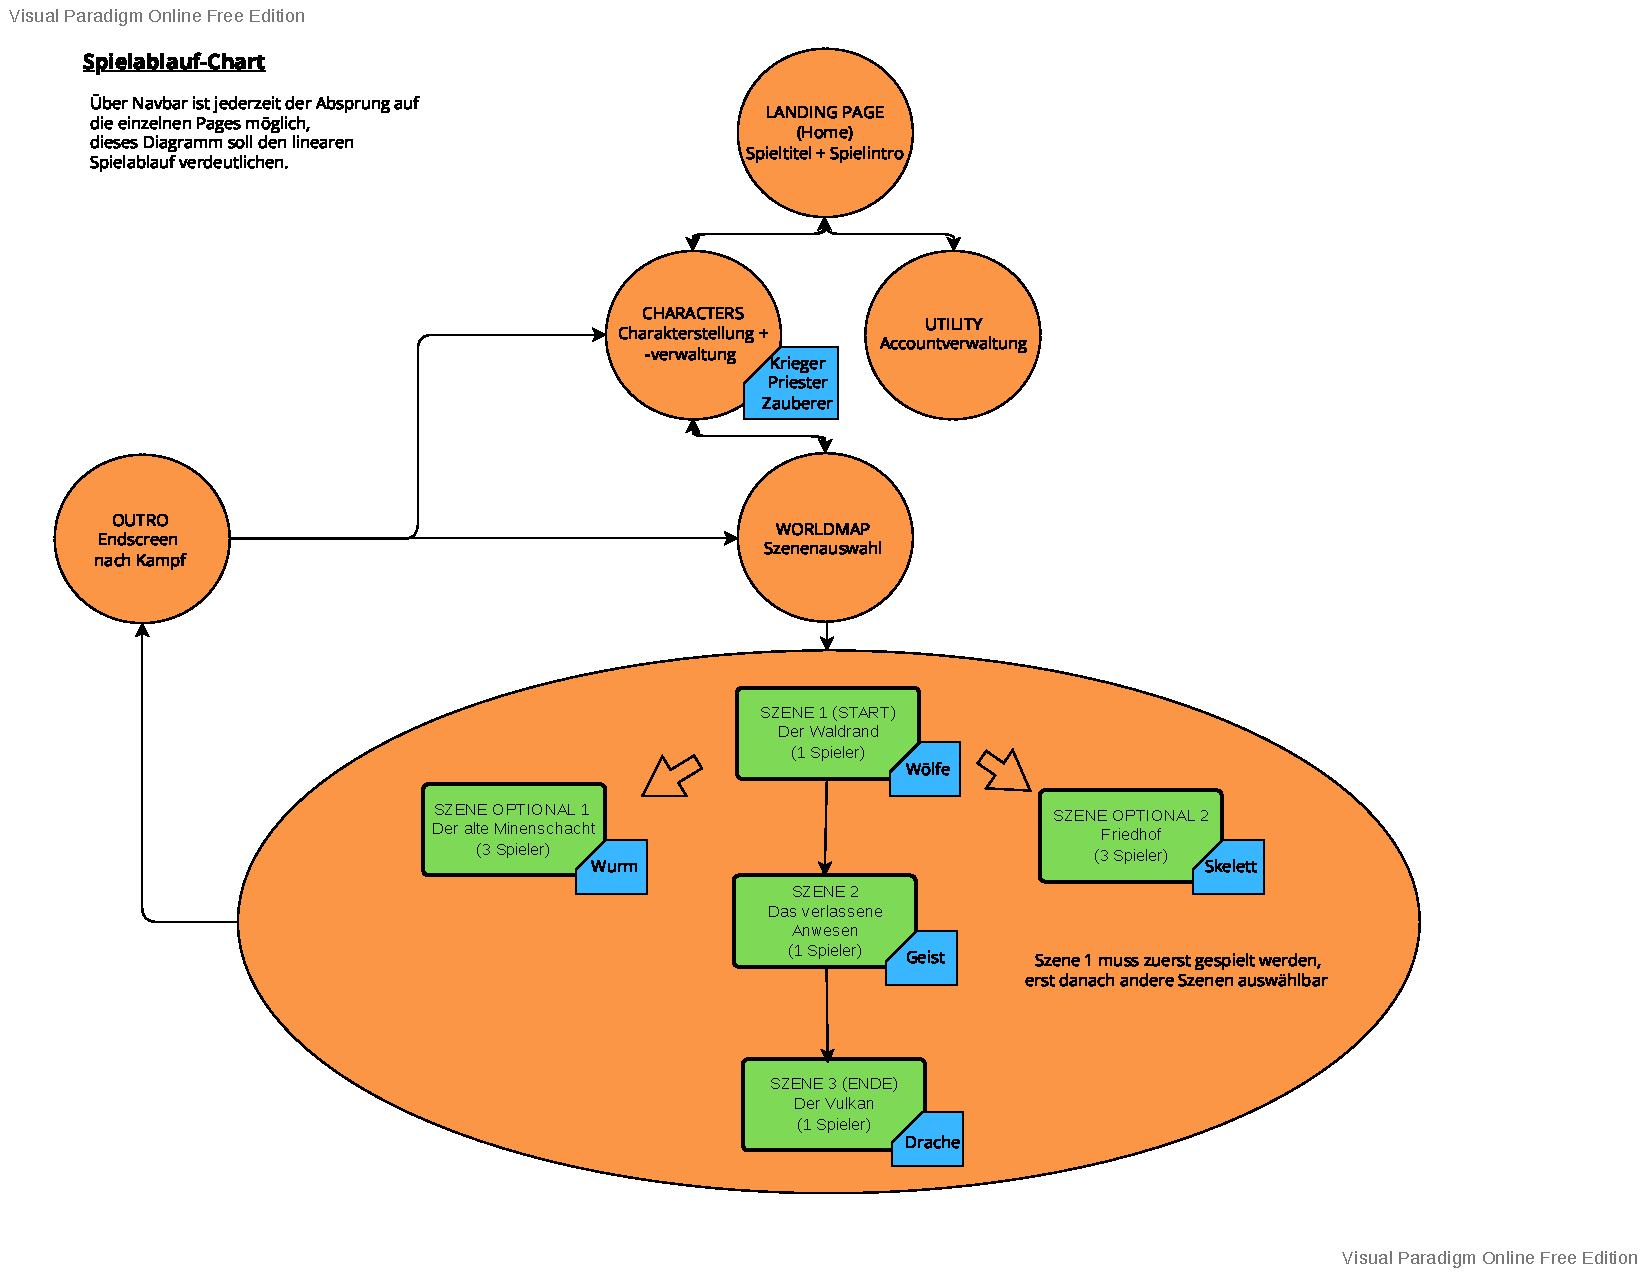
\includegraphics[width=1\textwidth, height=10cm]{2022-01-08-Spielablauf-Chart}
\end{figure}


\newpage


\section{Reflektion}
(TODO!): Jeder einen Punkt ausschreiben. 

3-4 gute Beispiele, max 1-2 Seiten

\begin{itemize}
    
    \item Umänderung Spielkonzept von Szenenbasiertem Gameplay (Verschiedene Wege, Adventuremäßig, Dialoge, ...) hin zu reinem Kampf-RPG.  
    
    \item Julian...

    \item \textbf{Rundenbasierter vs. chaotischer Spielablauf:} Der Ansatz die Entwicklung durch den Einsatz eines rundenbasierten Ablaufs bzw. Kampfsystems deutlich zu vereinfachen, muss wohl nach den Entwicklungen vom 27.12.2021 (\ref{ref-runden-impl}) zumindest angezweifelt werden. Denn der Aufwand, der durch die notwendige Konzeptionierung und Detailplanung entsteht ist nicht zu unterschätzen. Demengegen stünde bei einem chaotischen Spielablauf lediglich das Handling der Events. 

    \item \textbf{Kleinteilige Aufgabenpakete:} In der Entwicklung eine überschaubare Anzahl an kleinteiligen bzw. Teilufgaben vor sich zu haben, empfand Henning als sehr hilfreich. Man hat damit einen Überblick über die Arbeit der nächsten Tage. Bei der Entwicklung der Rundenlogik entstand durch die Kenntniss um die nächsten Rundenschritte hier ein stets guter Überblick. Der Abschluss jeder einzelnen Teil-Aufgabe sorgte weiter laufend für postive Motivation.

    \item \textbf{Lernkurve und Codequalität:} Eigentlich müsste am Ende eines Entwicklungs-Projektes stets noch einmal von vorne anfangen. Das allein um alles zu korrigieren und anzupassen bzw. auf einen gleichen Quaitätsstand zu bringen, was im Projektverlauf bei den Beteiligten an Fähigkeiten und Wissen gelernt wurde.
    

\end{itemize}






%-----------------------------------
% Apendix / Anhang
%-----------------------------------
\newcommand{\AppendixName}{Anhang}
\newpage
\section*{\AppendixName} %Überschrift "Anhang", ohne Nummerierung
\addcontentsline{toc}{section}{\AppendixName} %Den Anhang ohne Nummer zum Inhaltsverzeichnis hinzufügen

\begin{appendices}
% Nachfolgende Änderungen erfolgten aufgrund von Issue 163
\makeatletter
\renewcommand\@seccntformat[1]{\csname the#1\endcsname:\quad}
\makeatother
\addtocontents{toc}{\protect\setcounter{tocdepth}{0}} %
	\renewcommand{\thesection}{\AppendixName\ \arabic{section}}
	\renewcommand\thesubsection{\AppendixName\ \arabic{section}.\arabic{subsection}}
	


In diesem Abschnitt sind aktuell einige Unterlagen eingefügt, die im Rahmen des Projektes eine Relevanz hatten. Vor Abgabe der Projektarbeit, soll dieser Abschnitt überarbeitet, ausgedünnt und ergänzt werden. 

\section{Projektnotizen}

Austausch und Zusammenarbeite erfolgte auf verschiedenen Platformen:
\begin{itemize}
    \item Gezeichnet und Entwürfe wurden meist in Miro erstellt: \url{https://miro.com/app/board/uXjVOdN2haQ=/}. 
    \item Besprechungen erfolgten meist in Teams: \url{https://teams.microsoft.com/l/team/19%3aDoBvOwOIC6WNhsL9kOIYFKNtVftU1yBtcEn_gcyQtcg1%40thread.tacv2/conversations?groupId=850a22ff-34a2-4fe2-a506-f55ac4d595f8&tenantId=b9b6f99a-a243-422d-ab36-f726574c981a}. 
    \item Der gemeinsame Code und die Dokumentation wurden auf Github erstelt: \url{https://github.com/tstsrv-de/tstsrv-de}. 
\end{itemize}

\subsection{Projektbesprechungen}

Stets Sonntags erfolgten Projektbesprechungen. Notizen und Zusammenfassungen davon finden sich hier in fortschreitender, chronologischer Reihenfolge. Ebenso hier entsprechend einsortiert, finden sich Konzeptzeichnungen und Entwürfe aller Art (UI, Code, Datenbankmodelle).

(TODO!) Bildbeschreibungen ergänzen, wichtige Bilder beschreiben.

2021-11-23-erster-entwurf-gameloop 
\begin{figure}[H]
    \centering
    \caption[]{2021-11-23-erster-entwurf-gameloop}
    \label{fig:2021-11-23-erster-entwurf-gameloop}
    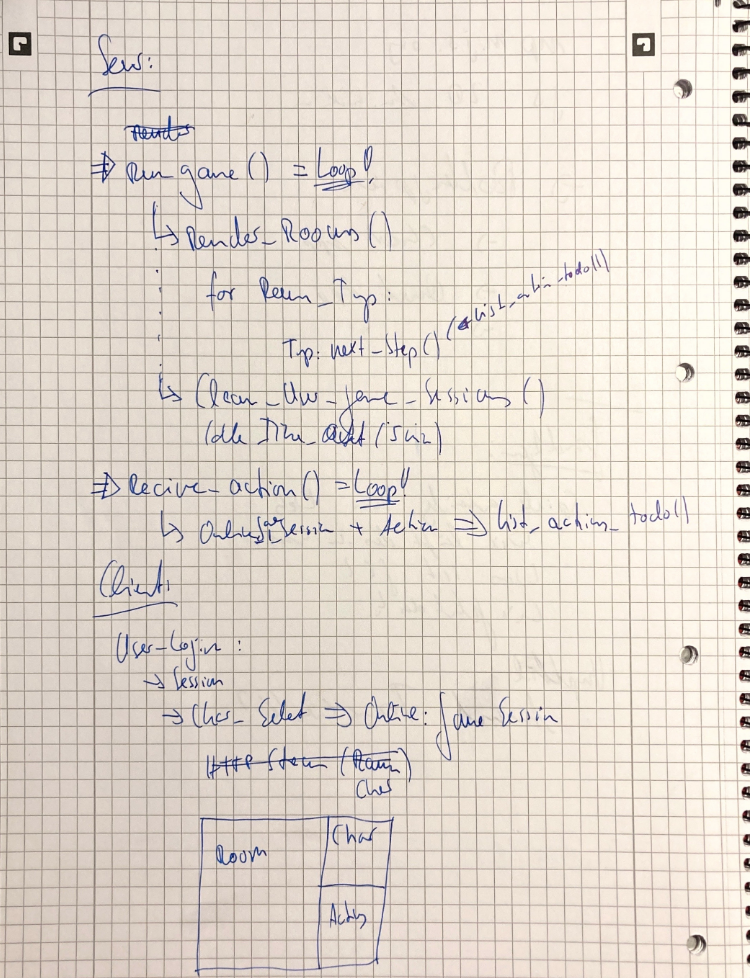
\includegraphics[width=1\textwidth]{2021-11-23-erster-entwurf-gameloop}
\end{figure}

2021-11-23-erstes-db-konzept 
\begin{figure}[H]
    \centering
    \caption[]{2021-11-23-erstes-db-konzept}
    \label{fig:2021-11-23-erstes-db-konzept}
    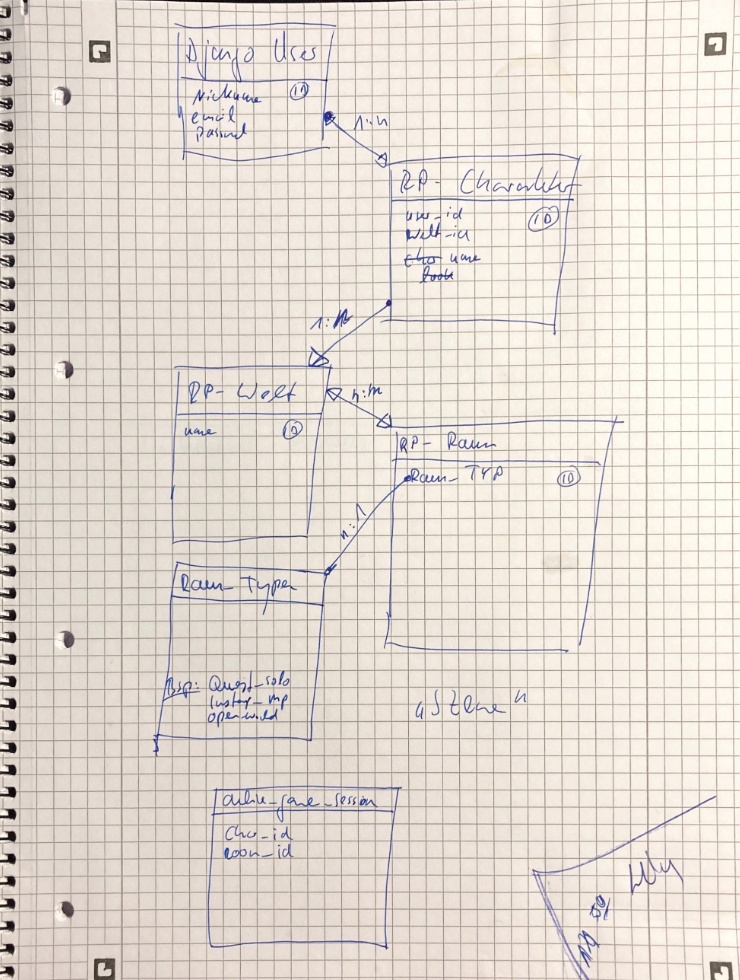
\includegraphics[width=1\textwidth]{2021-11-23-erstes-db-konzept}
\end{figure}

2021-11-27-erstentwurf-ui 
\begin{figure}[H]
    \centering
    \caption[]{2021-11-27-erstentwurf-ui}
    \label{fig:2021-11-27-erstentwurf-ui}
    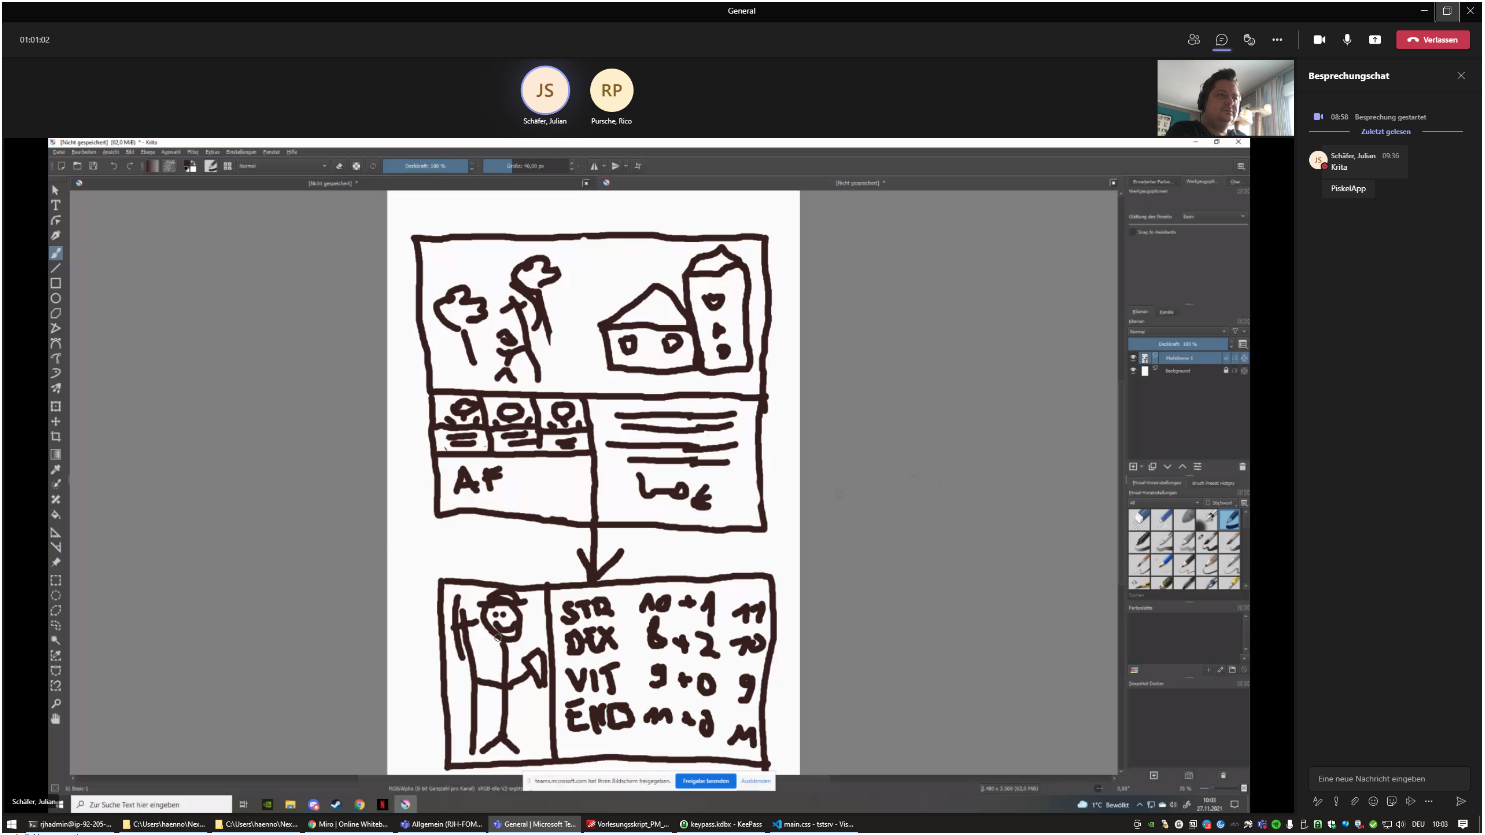
\includegraphics[width=1\textwidth]{2021-11-27-erstentwurf-ui}
\end{figure}

2021-11-27-projektskizze-1 
\begin{figure}[H]
    \centering
    \caption[]{2021-11-27-projektskizze-1}
    \label{fig:2021-11-27-projektskizze-1}
    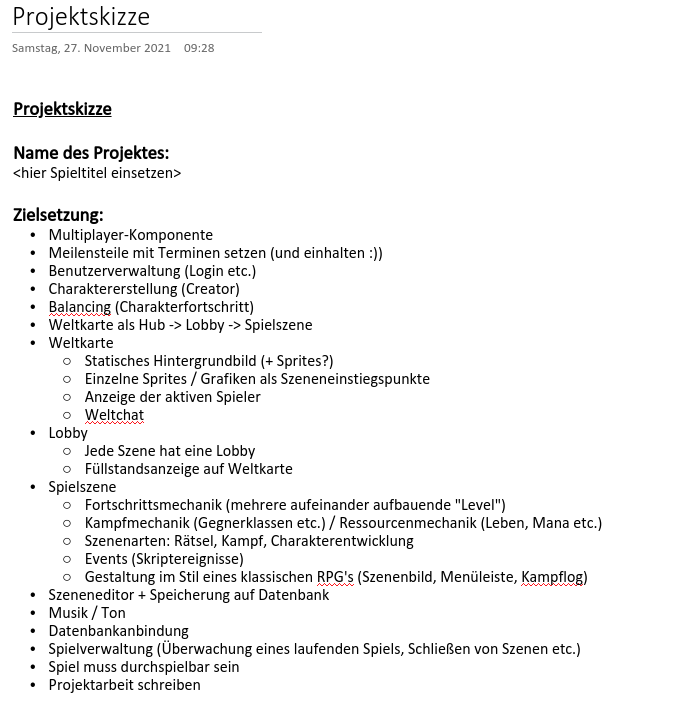
\includegraphics[width=1\textwidth]{2021-11-27-projektskizze-1}
\end{figure}

2021-11-27-projektskizze-2 
\begin{figure}[H]
    \centering
    \caption[]{2021-11-27-projektskizze-2}
    \label{fig:2021-11-27-projektskizze-2}
    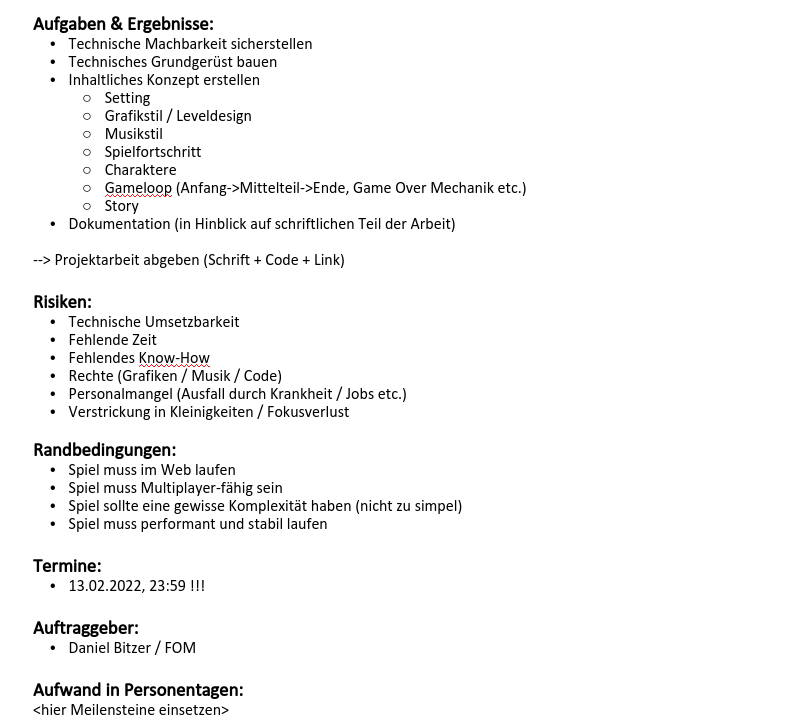
\includegraphics[width=1\textwidth]{2021-11-27-projektskizze-2}
\end{figure}

2021-11-29-Entwurf-Klassen-Ui 
\begin{figure}[H]
    \centering
    \caption[]{2021-11-29-Entwurf-Klassen-Ui}
    \label{fig:2021-11-29-Entwurf-Klassen-Ui}
    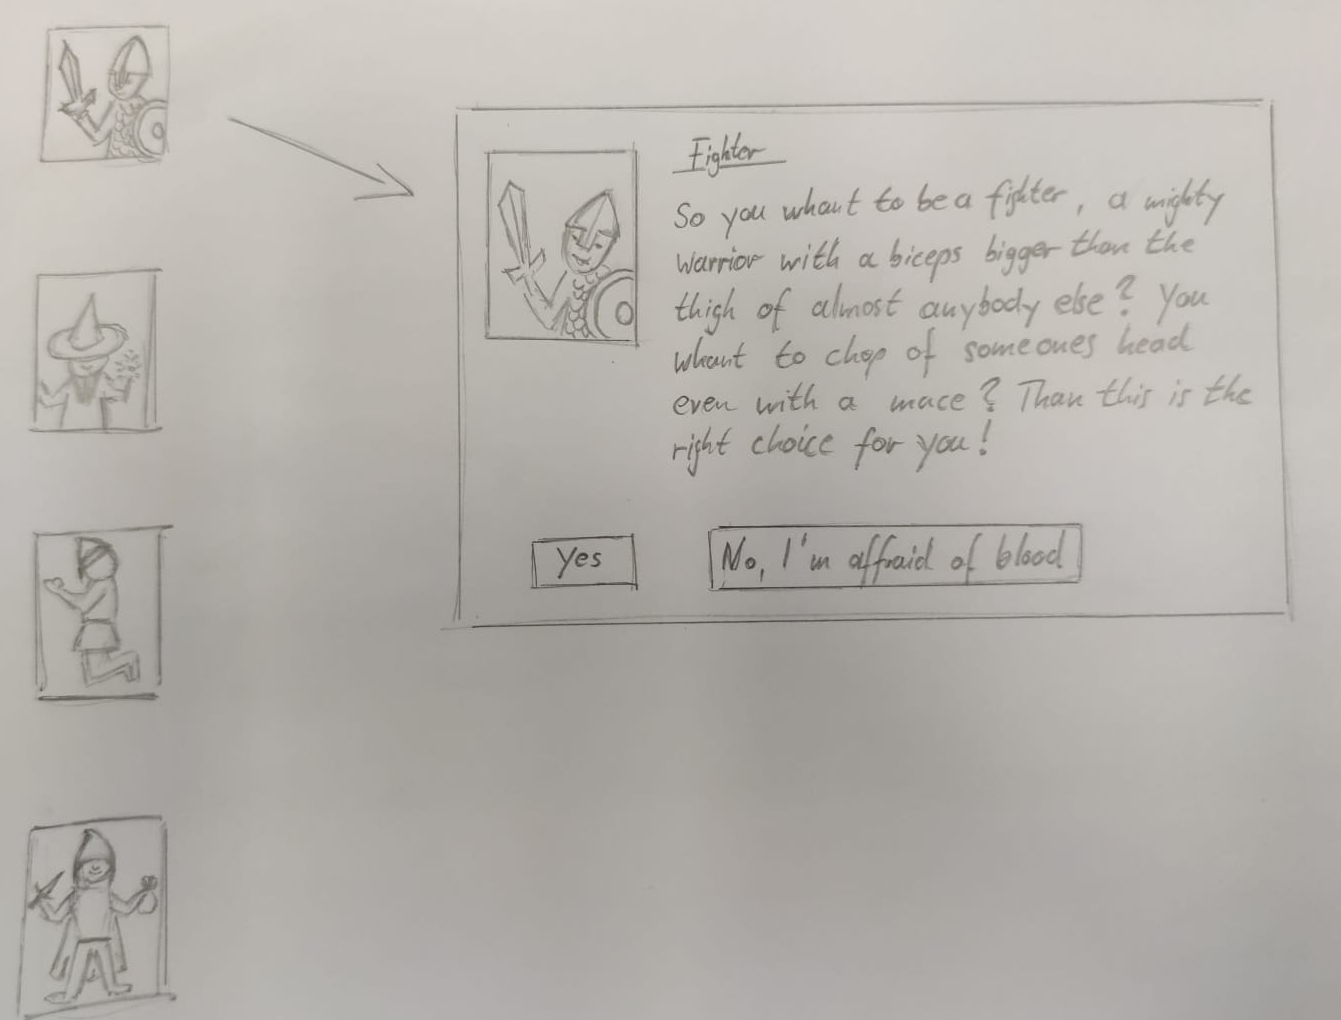
\includegraphics[width=1\textwidth]{2021-11-29-Entwurf-Klassen-Ui}
\end{figure}

2021-11-30-Entwurf-Lobby-Logik 
\begin{figure}[H]
    \centering
    \caption[]{2021-11-30-Entwurf-Lobby-Logik}
    \label{fig:2021-11-30-Entwurf-Lobby-Logik}
    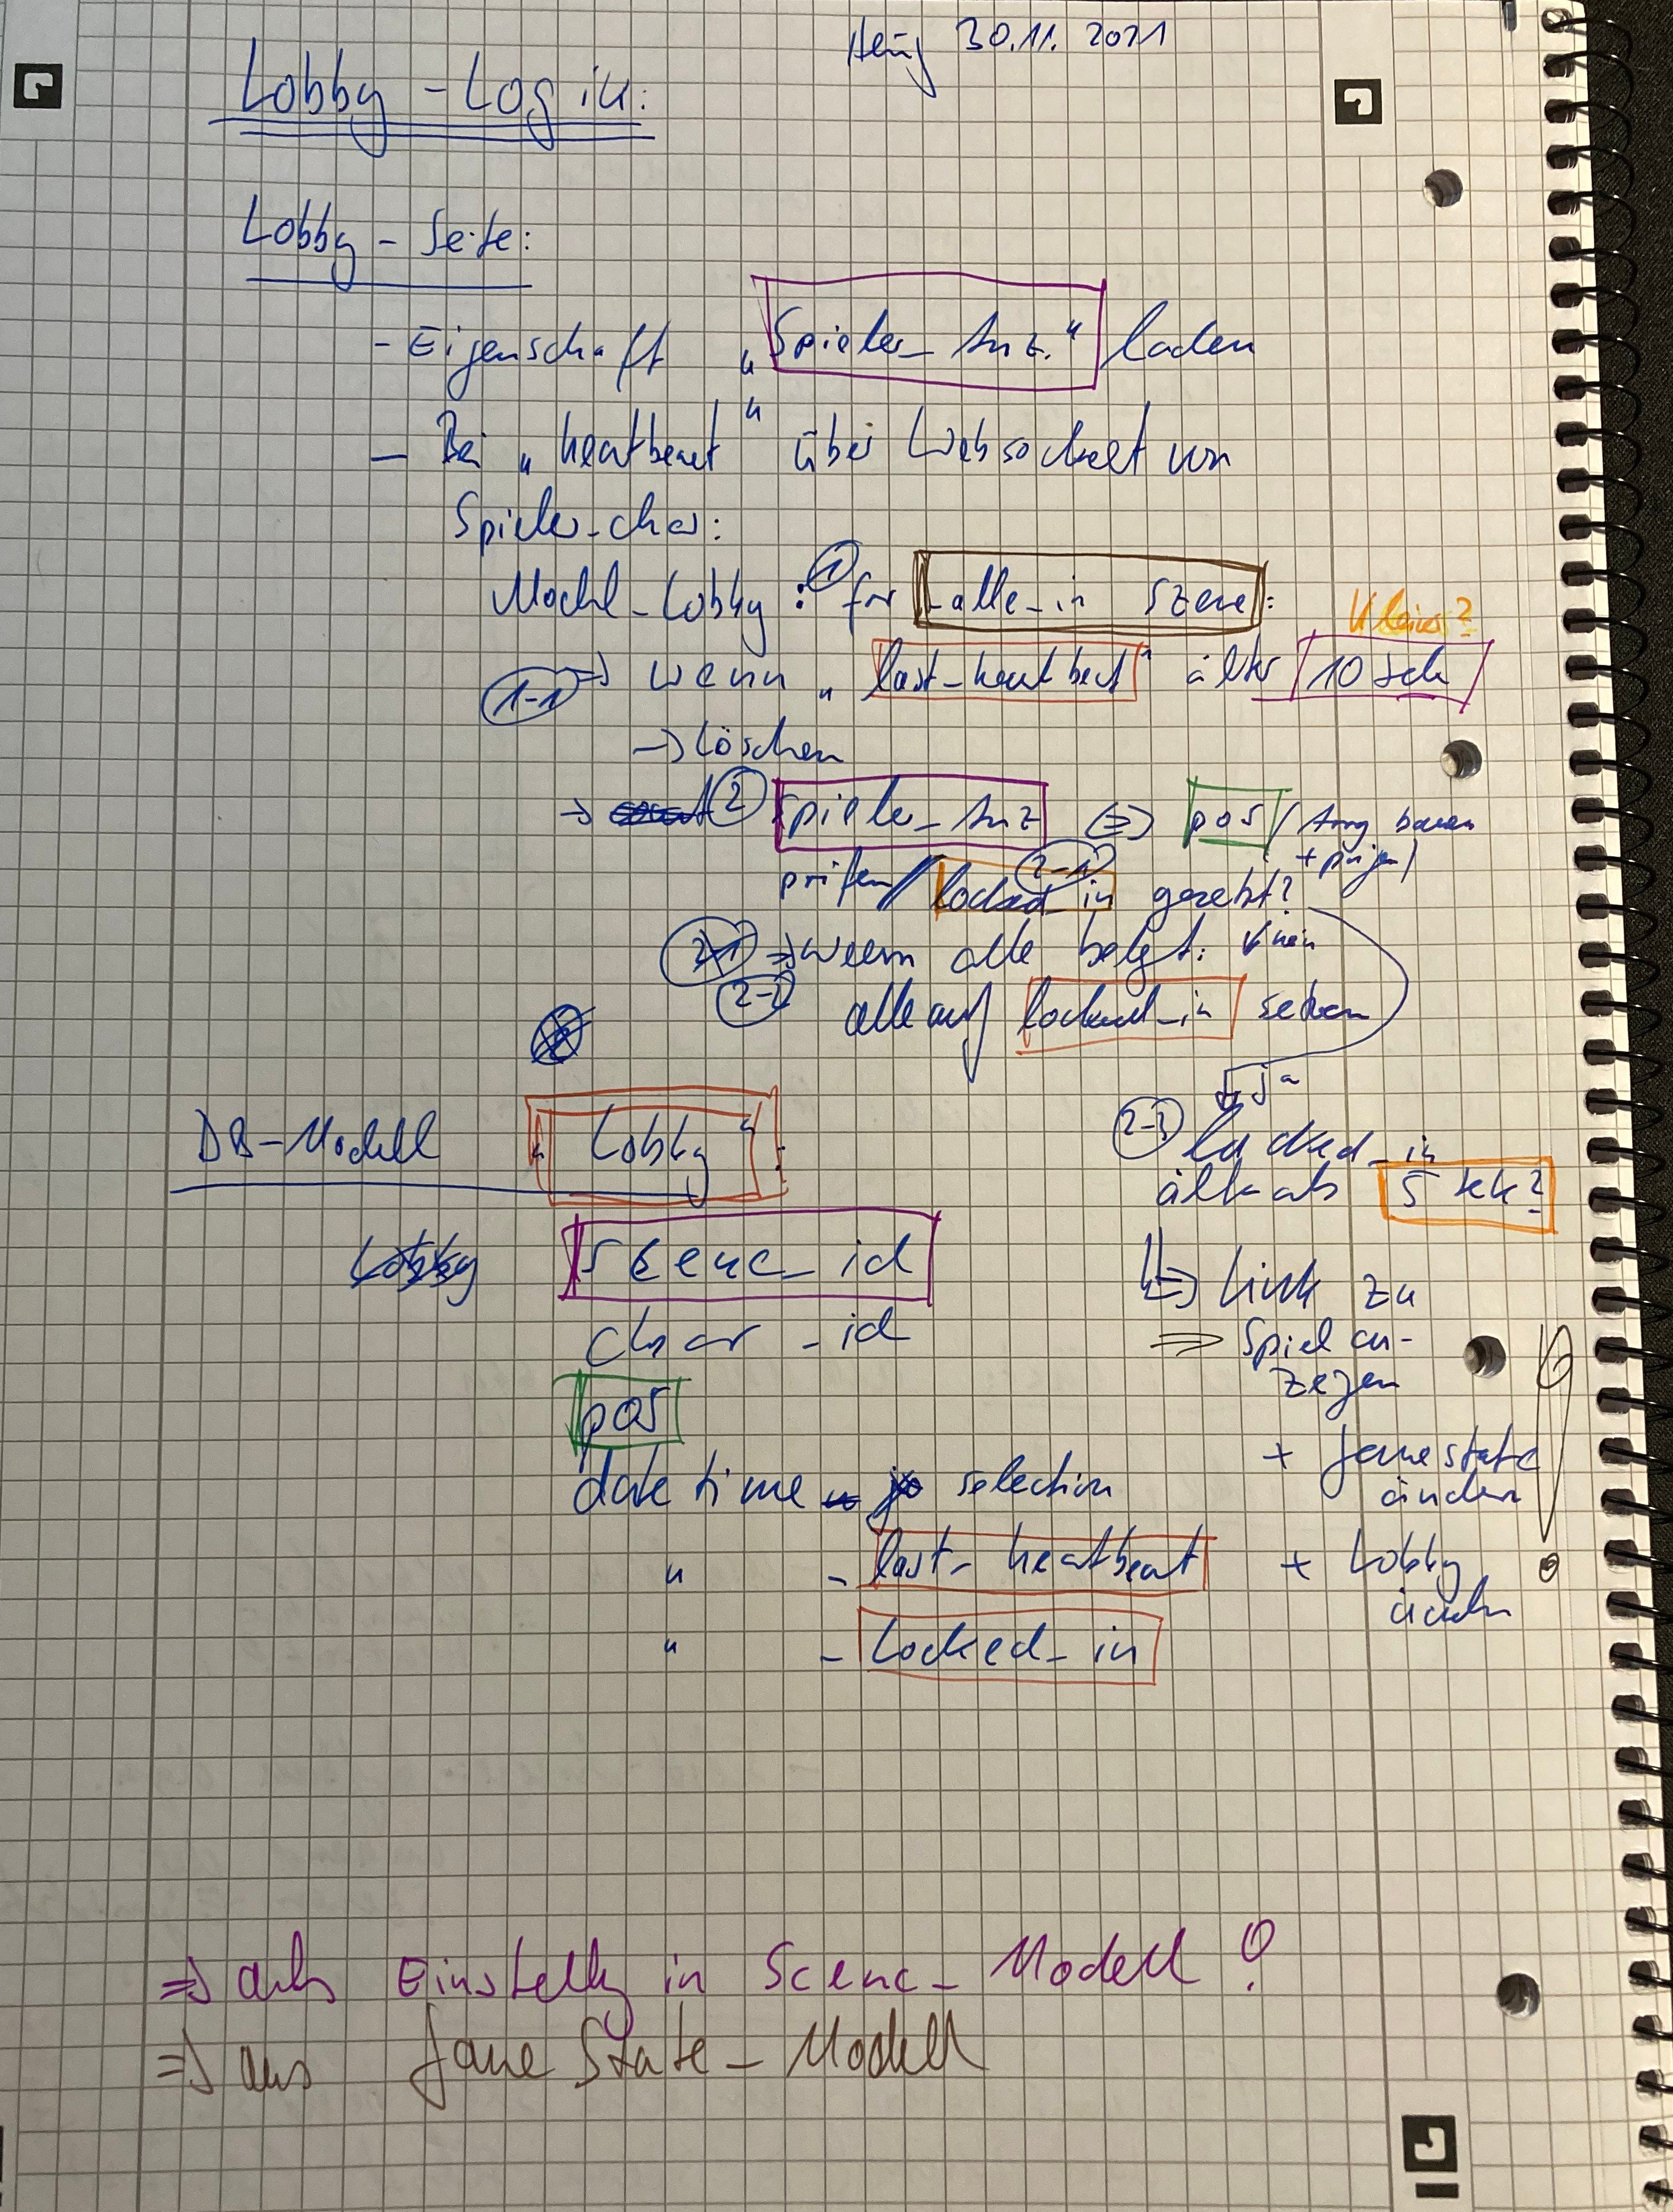
\includegraphics[width=1\textwidth]{2021-11-30-Entwurf-Lobby-Logik}
\end{figure}

2021-11-30-Entwurf-Lobby-UI 
\begin{figure}[H]
    \centering
    \caption[]{2021-11-30-Entwurf-Lobby-UI}
    \label{fig:2021-11-30-Entwurf-Lobby-UI}
    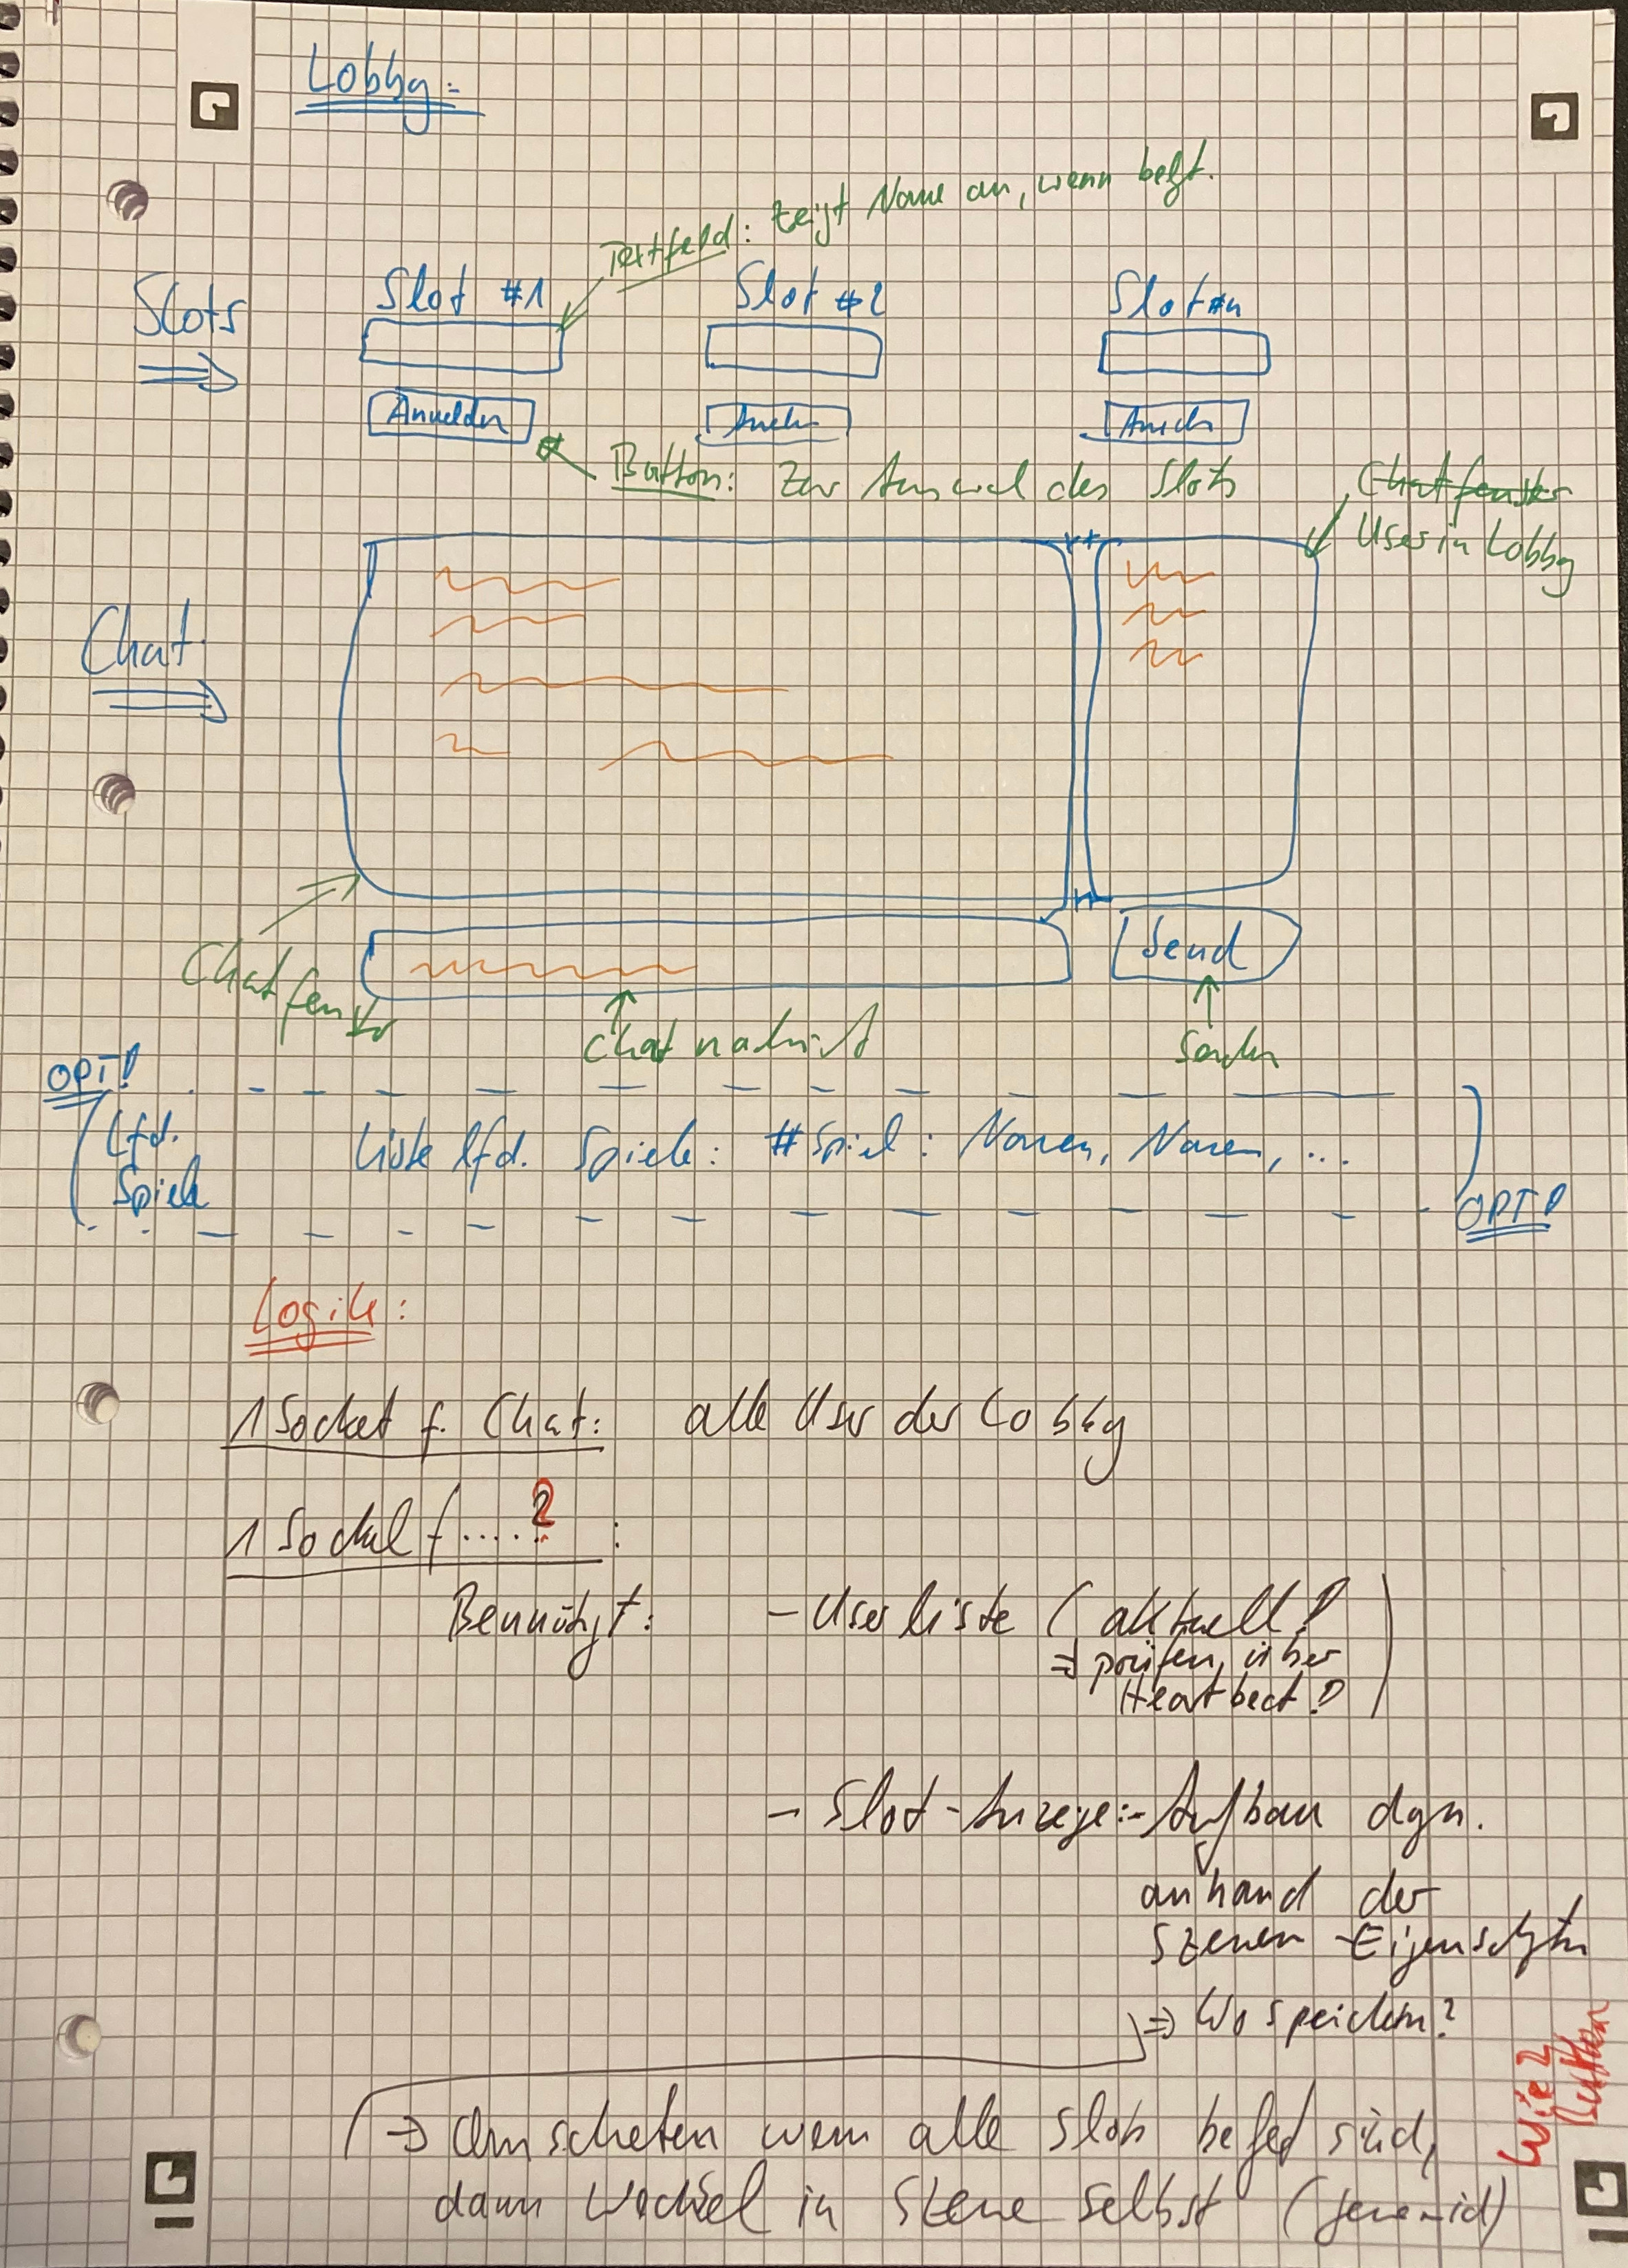
\includegraphics[width=1\textwidth]{2021-11-30-Entwurf-Lobby-UI}
\end{figure}

2021-12-02-Countdown-Logik 
\begin{figure}[H]
    \centering
    \caption[]{2021-12-02-Countdown-Logik}
    \label{fig:2021-12-02-Countdown-Logik}
    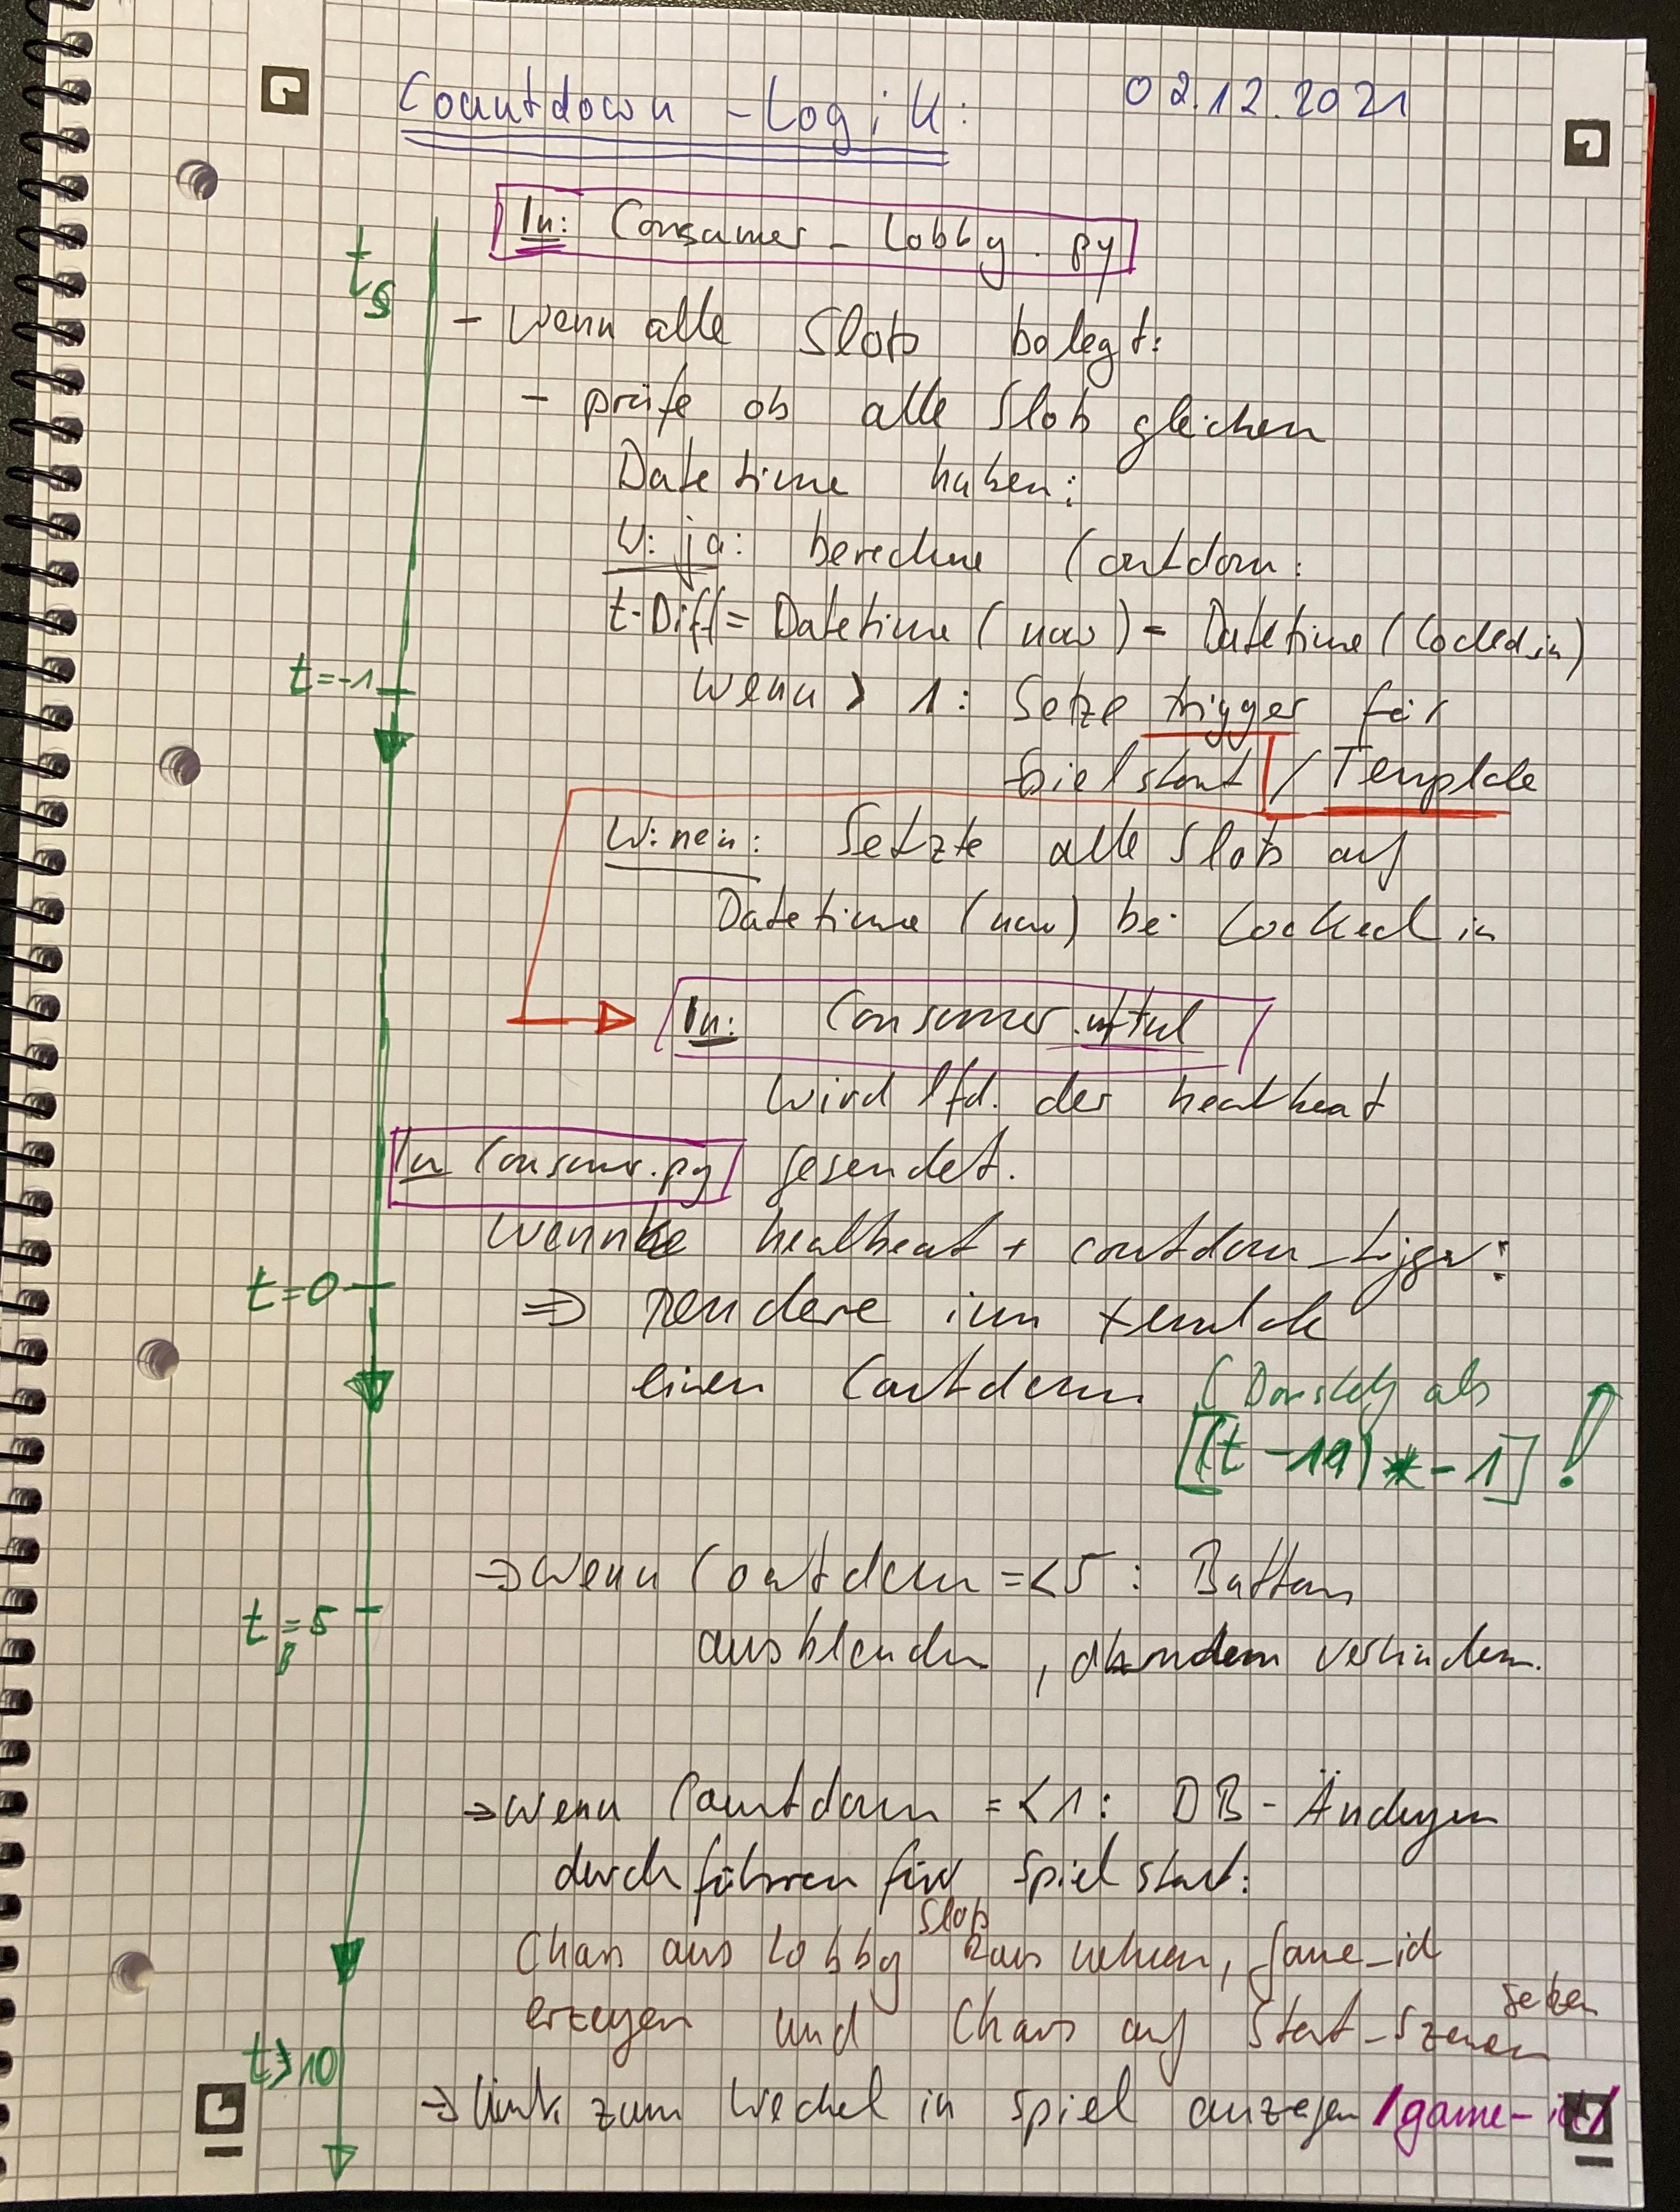
\includegraphics[width=1\textwidth]{2021-12-02-Countdown-Logik}
\end{figure}

2021-12-05-Projketbesprechung-Miro-b 
\begin{figure}[H]
    \centering
    \caption[]{2021-12-05-Projketbesprechung-Miro-b}
    \label{fig:2021-12-05-Projketbesprechung-Miro-b}
    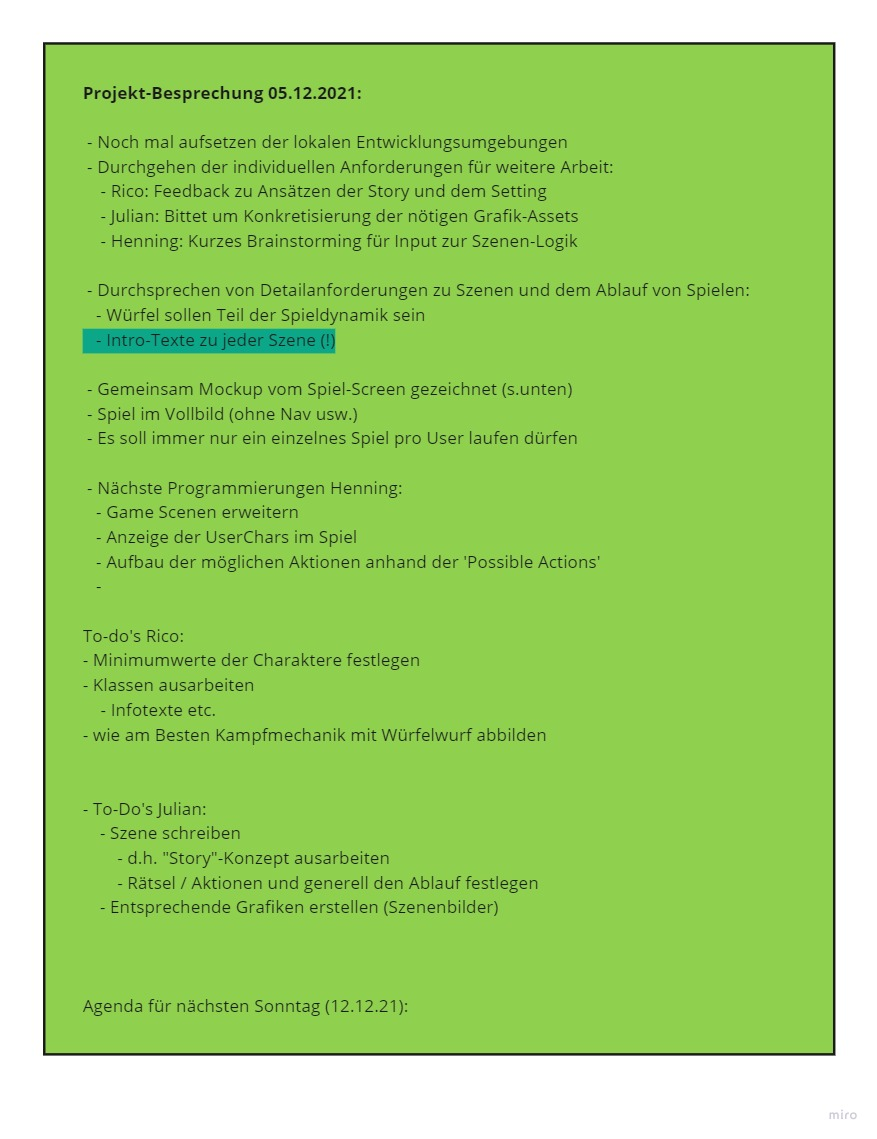
\includegraphics[width=1\textwidth]{2021-12-05-Projketbesprechung-Miro-b}
\end{figure}

2021-12-05-Projketbesprechung-Miro-c 
\begin{figure}[H]
    \centering
    \caption[]{2021-12-05-Projketbesprechung-Miro-c}
    \label{fig:2021-12-05-Projketbesprechung-Miro-c}
    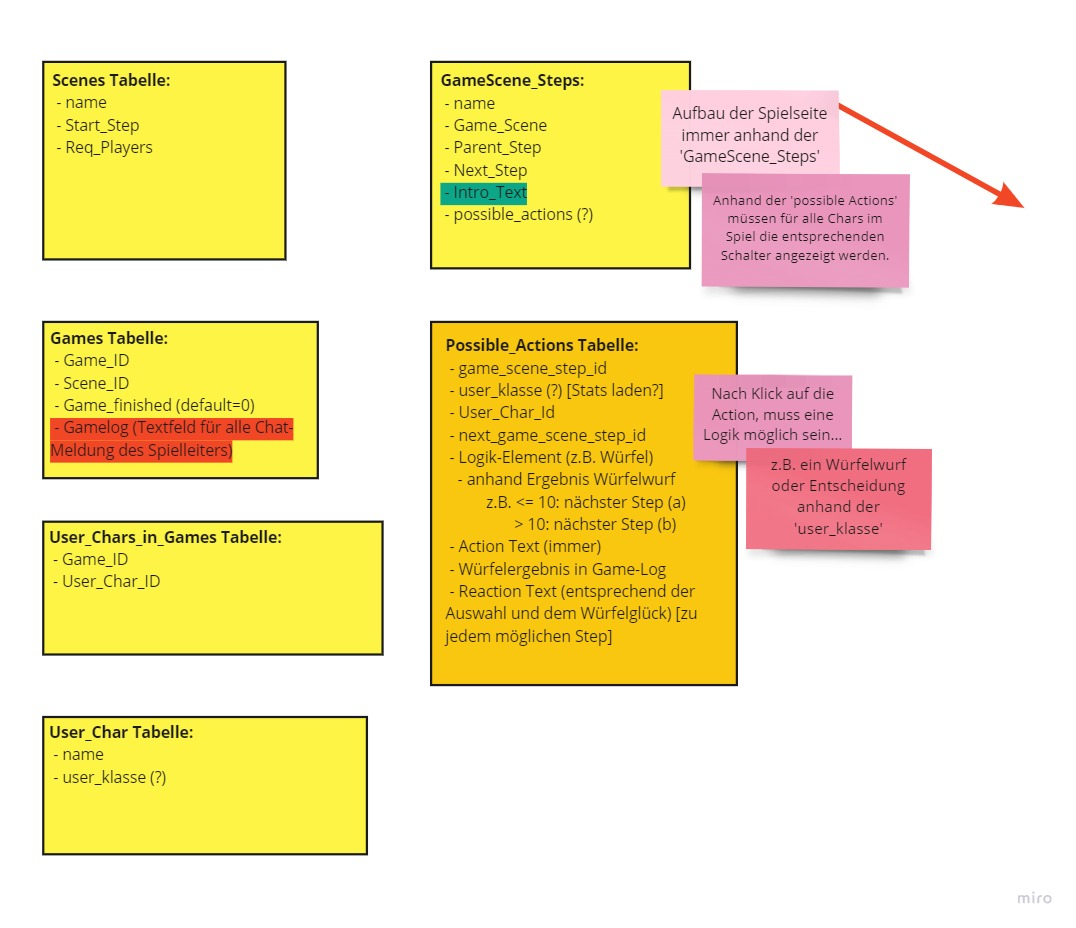
\includegraphics[width=1\textwidth]{2021-12-05-Projketbesprechung-Miro-c}
\end{figure}

2021-12-05-Projketbesprechung-Miro-d 
\begin{figure}[H]
    \centering
    \caption[]{2021-12-05-Projketbesprechung-Miro-d}
    \label{fig:2021-12-05-Projketbesprechung-Miro-d}
    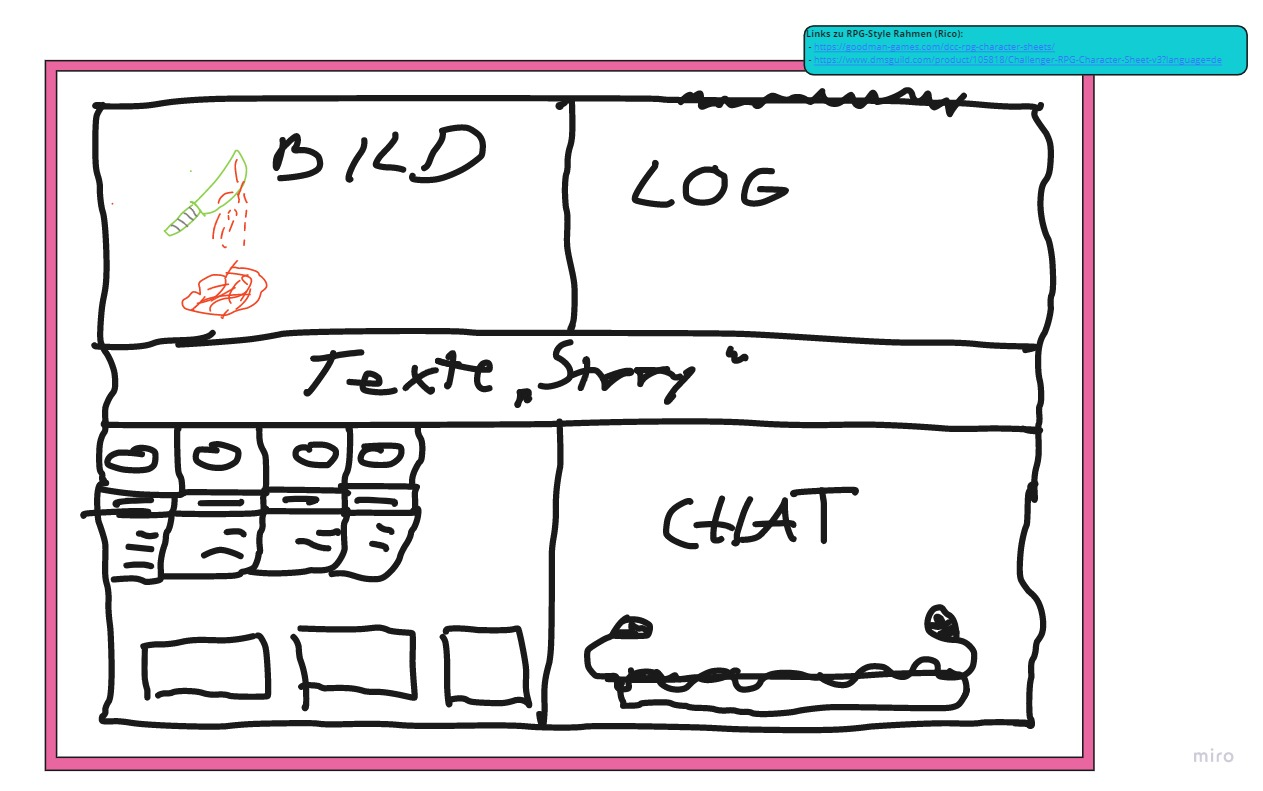
\includegraphics[width=1\textwidth]{2021-12-05-Projketbesprechung-Miro-d}
\end{figure}

2021-12-11-Projekt-Besprechung-Klassenbeschreibung 
\begin{figure}[H]
    \centering
    \caption[]{2021-12-11-Projekt-Besprechung-Klassenbeschreibung}
    \label{fig:2021-12-11-Projekt-Besprechung-Klassenbeschreibung}
    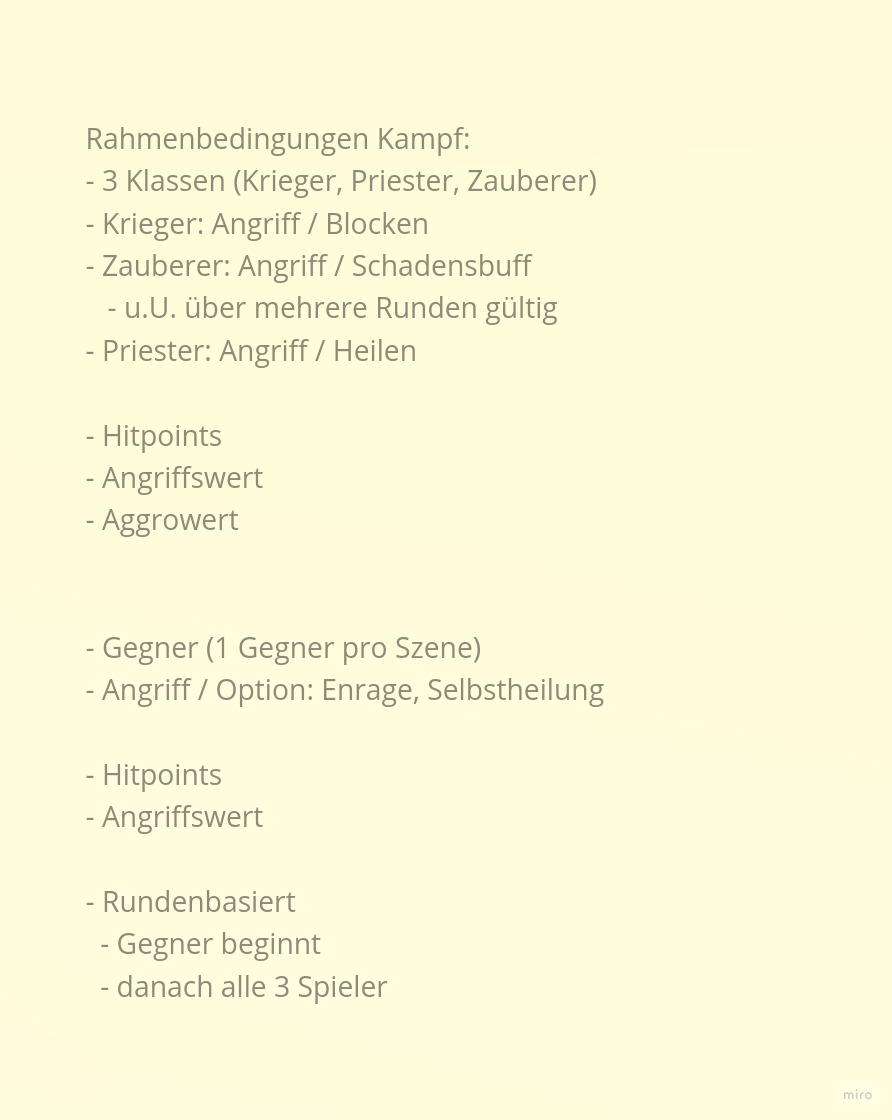
\includegraphics[width=1\textwidth]{2021-12-11-Projekt-Besprechung-Klassenbeschreibung}
\end{figure}


\begin{figure}[H]
    \centering
    \caption[]{11.12.2021: Projekt Besprechung: Gegenseitiges Update und Wechsel von Szenenlogik zu Kampfsystem für das RPG }
    \label{fig:2021-12-11-Projekt-Besprechung}
    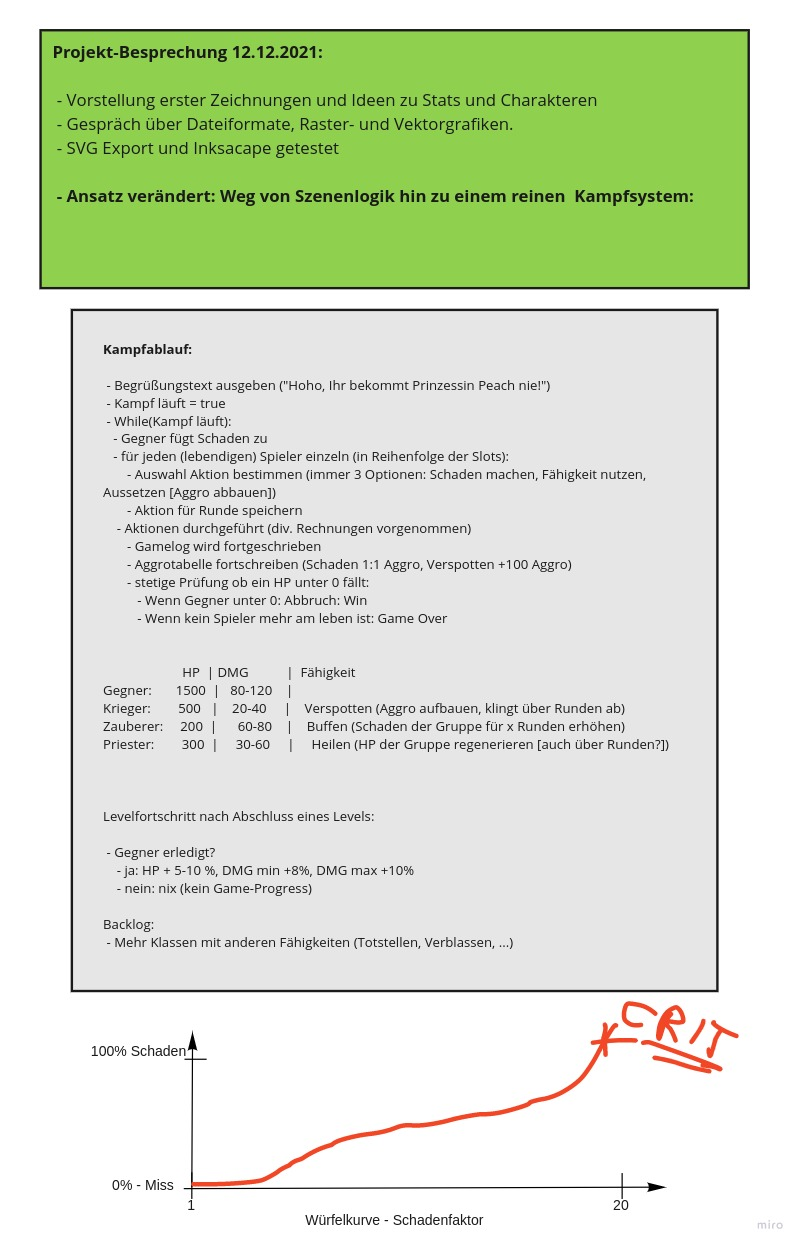
\includegraphics[width=1\textwidth]{2021-12-11-Projekt-Besprechung}
\end{figure}



\section{Entwicklungsnotizen}

\subsection{Entwicklung, Sonntag 19.12.2021:}

An diesem Tag wurden weitere, notwenige Grundlagen für die Integration der Spiellogik eingebaut. Das insbesondere in Vorbereitung auf die kommenden Anpassungen und Entwicklungen die in der Projektbesprechung vom 11.12.2021 besprochen wurden. 
Konkret: 

\begin{itemize}
	\item Prüfung auf den Seiten Chars, Worldmap und Lobby ob dieser Benutzer ein aktives Spiel hat. Falls ja, wird der Benutzer auf diese Seite umgeleitet.
	\item Grundfunktion für das Beenden von einem Spiel eingebaut: Man kann nun per Klick im Spiel, das Spiel beenden.
	\item Daran anschließend eine Prüfung im laufendem Spiel, ob das Spiele beendet wurde und falls ja, Anzeige eines Endbildschirms.
\end{itemize}

Die Entwicklung der Grundlagen an diesem Tag wurde mit Fokus auf Modularisierung erledigt. Der Code der jeweiligen Funktionen wurde in einzelnen Dateien ausgelagert um Wiederverwendbarkeit und Lesbarkeit zu erhöhen. 

Die zugehörigen Commits sind insbesondere: 
\url{https://git.io/JDjKl} und 
\url{https://git.io/JDjKB}


\subsection{Entwicklung, Dienstag 21.12.2021:}

Grundlagen des Kampfsystems entsprechend der Projekt-Besprechung vom 11.12.2021 (Abbildung \ref{fig:2021-12-11-Projekt-Besprechung}) sollen implementiert werden.

Vorbereitungen: 

\begin{itemize}
    \item Tabelle "GamesScenesSteps" und Verknüpfungen entfernen (Commits \url{https://git.io/JDjKz} und \url{https://git.io/JDjKg})
    \item Kampf-/Gamelog erzeugen: Darin werden alle Meldungen aus dem Spiel wie z.B. Kampftexte, Schaden, Aktionen, Systemmeldungen und alles andere denkbare angezeigt und gespeichert. Getrennt davon soll der Chat-Log dargestellt werden. Dazu werden in der Tabelle "Games" zwei neue Textfelder erzeugt (Commit \url{https://git.io/JDj63}). 
    \item Anzeige des Game-Logs auf der Spielseite. Schreiben von Nachrichten in das Gamelog als ersten Test des grundlegend umgestellten Seitenaufbaus: Es werden nur noch einzelene Elementinhalte per Websocket transportiert, nicht mehr ganze HTML-Code-Blöcke (Commit \url{https://git.io/JyeJQ}).
\end{itemize}


\subsection{Entwicklung, Montag 27.12.2021:}

Weitere Entwicklungen entsprechend der Projekt-Besprechung vom 11.12.2021 (Abbildung \ref{fig:2021-12-11-Projekt-Besprechung}):

\begin{itemize}
    \item Eintrag ins Gamelog zum Spielstart (Commit \url{https://git.io/JyBRf}).
    \item Rundensystem implementieren. Dazu mindestens notwendig: Lebens- und Angriffspunkte der User-Chars sowie des Gegners.
\end{itemize}



	% 




\section{Aufgabenbeschreibung}
Beispielinhalt und Texte:
Das Thema der Seminararbeit gründet als Idee vor allem aus den folgenden beiden Beobachtungen aus privatem Lebensalltag und beruflicher Praxis: 
\begin{enumerate}
	\item Die seit den 2010er Jahren aufkommenden \textbf{smarten Technologien} finden im öffentlichen Raum und im Lebensalltag breiter Bevölkerungsschichten immer mehr Einzug. Drei Anwendungsbeispiele verdeutlichen und belegen das: 
	\begin{itemize}
	 \item Smart Watch: Uhren die z.B. um Fitness- und Nachrichtenfunktionen erweitert sind.
	 \item Smart TV: Fernsehgeräte die z.B. Zugriff auf Internet-Mediatheken erlauben.
	 \item Smart Home: Hausautomatisierungen und -steuerungen im privaten Bereich für  z.B. Licht und Heizung.
	 \end{itemize}

	 \item Das Aufkommen und der Erfolg der \textbf{PropTech\footnote{Kofferwort, englisch, aus 'property' (Immobilien) und 'technology' (Technologiegen)}-Branche} sowie die dieser Branche zuzuordnenden Unternehmen belegt die Relevanz von Innovation für die Wohnungswirtschaft ebenso wie die folgenden Erkenntnisse einer Studie \parencite[S. 18]{zia}:
	 \begin{itemize}
		 \item 72\% der befragten immobilienwirtschaftlichen Unternehmen nehmen Effizienzsteigerungen in Kernprozessen durch Einsatz digitaler Technologien an.
		 \item Weiter: Über ein Drittel gehen davon aus, dass Neugeschäft durch Einsatz digitaler Technologien generiert werden kann. 
	 \end{itemize}
\end{enumerate}

Vorgenannte Beobachtungen führen zu folgender Hypothese:

 \Rightarrow \textbf{Der Einsatz von smarten Displays in Quartieren der \ac{WoWi} ist möglich, wirtschaftlich und innovativ.}



\subsection{Was ist das Ziel der Projektarbeit?}
Beispielinhalt und Texte:
Als mögliche Standorte ergeben sich in Anlehnung an bisher übliche \glqq{}schwarze Bretter\grqq{} und \glqq{}Schaukästen\grqq{} in den Gebäuden sowie auch im Außenbereich vorhandenen Anlagen (Schaukästen, Werbeanlagen) auch für smarte Displays einige Vor- und Nachteile (Pro und Contra) die wie folgt stichpunktartig beschrieben werden: 

 \begin{itemize}
	 \item \textbf{Innenbereich:} 
	 \\ Wandmontage ebenso wie üblich und bekannte Schaukästen und schwarze Bretter im Windfang oder dem Etagenflur im Erdgeschoss eines Mietshauses.\\
	 \textbf{Pro:}\\
	  - Weiternutzung vorhandener, bewährter Montageorte \\
	  - Baurechtlich genehmigungsfrei \\
	  - Anbindung an Strom und Internet leichter als im Außenbereich \\
	  - Günstigere Bauart (kann weniger witterungsfest und vandalismussicher sein)\\
	 \textbf{Contra:}\\
	  - Wird wenig innovative Bauart zur Folge haben\\
	  - Kleinere Anzeigeflächen \\
	  - Nutzerkreis umfasst nur Mieter und Besucher des Hauses
	 \item \textbf{Außenbereich:} 
	 \\ Als freistehende Installation vor einem Wohngebäude, an einem markanten Wegepunkt im Quartier oder einem Innenhof eines Gebäudekomplexes.\\
	 \textbf{Pro:}\\
	  - Höhere Sichtbarkeit und Reichweite (nicht nur Mieter und Besucher eines Hauses, sondern auch Umfeld, Nachbarn und Durchgangsverkehr)  \\
	  - Attraktive Bauarten möglich \\
	  - Eröffnet weitergehende Nutzungsmöglichkeiten \\
	 \textbf{Contra:}\\
	  - Höhere Investitionskosten durch dem Standort geschuldete Bauart und Größe \\
	  - Erdarbeiten werden in der Regel nötig sein (Stromanschluss)  \\
	  - Baurechtlich genehmigungspflichtig, verursacht Mehrkosten und Aufwand
	  \item \textbf{Übergangsbereich Hauseingangstüre:} 
	  \\ Anbringung an Flächen die das Gebäude und den Außenbereich verbinden, beispielhaft genannt hier: Seitenteil der Türelemente im Hauseingangsbereich.\\
	  \textbf{Pro:}\\
	   - Unter Umständen umsetzbar als Modernisierungsmaßnahme (Nutzung als Videogegensprechanlage)  \\
	   - Technikaverse Bewohner und Besucher kommen zwangläufig in Kontakt mit dem smart Display \\
	  \textbf{Contra:}\\
	   -  Vorteile ergeben sich z.T. nur in noch nicht modernisiertem Bestand \\
	   -  Kleinerer Nutzerkreis und Anzeigefläche \\
 \end{itemize}

Eine weitergehende Bewertung oder Befürwortung einzelner Standorte soll hier nicht erfolgen um einzelne Anwendungsfälle nicht hier schon auszuschließen.


\subsection{Worin bestehen die (wahrscheinlichen) Herausforderungen? (allg. technisch und auch persönlich)}
Beispielinhalt und Texte:
Der Begriff soll daher hier geschärft werden um in der weiteren Verwendung un­miss­ver­ständ­lich zu sein.  

Die Definition erfolgt unter Bezug auf
\begin{enumerate}
	\item  die erfolgte Abgrenzung in 'enge' und 'weite' Definition nach \citeauthor{wirtschaftsfaktorimmo} (\citeyear[S. 9]{wirtschaftsfaktorimmo}) sowie
	\item die institutionelle Systematisierung der Immobilienwirtschaft nach \citeauthor{brauer2011einfuhrung} (\citeyear[S. 26]{brauer2011einfuhrung}).
\end{enumerate}

Die daraus entnommenen Zitate sollen hier im weiteren als gültige Definition für den verwendeten Begriff \textbf{Wohnungswirtschaft (WoWi)} gelten:  
\begin{itemize}
	\item Aus \citeauthor{wirtschaftsfaktorimmo} (\citeyear[S. 9]{wirtschaftsfaktorimmo}): \glqq{}alle Unternehmen, die an der Bewirtschaftung, Vermittlung und Verwaltung von Immobilien unmittelbar beteiligt sind\grqq{}. 
	 \item Sowie nach \citeauthor{brauer2011einfuhrung} (\citeyear[S. 36]{brauer2011einfuhrung}) zu den unterschiedlichen Rechtsformen \glqq{}(...)kommunalen, genossenschaftlichen und privaten Unternehmen(...)\grqq{} und den gleichwohl identischen Aufgabenfeldern: \glqq{}(...)nachhaltige Vermietung und Bestandsmanagement(...)\grqq{}.
\end{itemize}





\newpage
\section{Anforderungen}
Beispielinhalt und Texte:
Die genaue Zuordnung stellt sich also wie folgt dar:

\begin{table}[H]
	\caption{Zuordnung der Anforderungen der Hypothese zu den kritischen Anforderungen des Proof of Concept (PoC)}
	\label{tbl:zuordnungHypothesePoc}
	\begin{tabularx}{\textwidth}[ht]{|l|c|X|}
	\hline
	\textbf{Anforderung der Hypothese} & \textbf{Zuordnung} & \textbf{Abbildung in \ac{PoC}} \\
	\hline\hline 
	ist möglich & \Leftrightarrow & Prüfung der Machbarkeit  \\
	\hline 
	ist wirtschaftlich & \Leftrightarrow &  Effizienz-Faktoren aufzeigen \\
	\hline 
	ist innovativ & \Leftrightarrow &  Nutzbarkeit und Anwendungsfälle \\
	\hline
	\end{tabularx}
\end{table}


\subsection{Welche Techniken/ Technologien sollen eingesetzt werden, um die Aufgabe zu lösen/ realisieren?}
Beispielinhalt und Texte:

Eine Betrachtung der Wirtschaftlichkeit einer Einzelinvestition in ein smart Display in einem Quartier könnte damit nach z.B. folgendem Schema erfolgen:


\begin{table}[H]
	\caption{Mögliches Schema einer Wirtschaftlichkeits- und Effizienzbetrachtung der Einzelinvestition in smart Displays}
	\label{tbl:SchemaWBsmartDisplay}
	\begin{tabularx}{\textwidth}[ht]{cl}
	\hline
	\textbf{ - }   &  Investitionskosten (der Einzelmaßnahme) \\
	\textbf{ - }   &  lfd. Betriebs- und Wartungskosten  \\
	\textbf{ + }   &  lfd. Einsparung Personalkosten  \\
	\textbf{ + }   &  Refinanzierung als Modernisierungsmaßnahme   \\
	\textbf{ + }   &  Umlage von (Teilen der) Betriebskosten auf Gebäudenutzer  \\
	\textbf{ + }   &  Mehrerlöse durch Überlassung als Werbefläche an Dritte  \\
	\hline\hline
	\textbf{ = }   &  \textbf{in Euro messbare Wirtschaftlichkeit} \\
	\textbf{ + }   &  Digitalisierung eines Geschäftsprozesses  \\
	\textbf{ + }   &  Imagegewinn für das Quartier \\
	\textbf{ + }   &  Öffentlichkeitswirksame Einführung und Realisierung  \\
	\hline\hline
	\textbf{ = }   &  \textbf{gesamt zu bewertende Effizienz} \\
	\hline
\end{tabularx}
\end{table}

Kommt man nun zurück auf die Definition des Bergriffs der Effizienz nach \citeauthor{eichhorn2016} (\citeyear[S. 183 f.]{eichhorn2016}), kann man feststellen, dass es für die Beurteilung wesentliche Faktoren gibt, die nicht der Wirtschaftlichkeit zuzurechnen sind.



\subsection{Warum sollen gerade diese eingesetzt werden?}
Beispielinhalt und Texte:
Mit smarten Displays sind in dieser Seminararbeit nicht die von Desktop-Computer abnehmbaren und tragbaren LCD-Monitore gemeint die 2002 im Zusammenhang mit Microsofts Betriebssystem \glqq{}Windows CE for Smart Displays\grqq{} vorgestellt wurden \parencite{heise-ms-sd} und im Jahr 2004 wieder eingestellt worden sind \parencite{ct-3-2004}. 

\begin{figure}[H]
	\caption{Handteil eines smart Displays nach Microsoft-Konzept}\label{fig:HandteilMSsmartDisplay}
	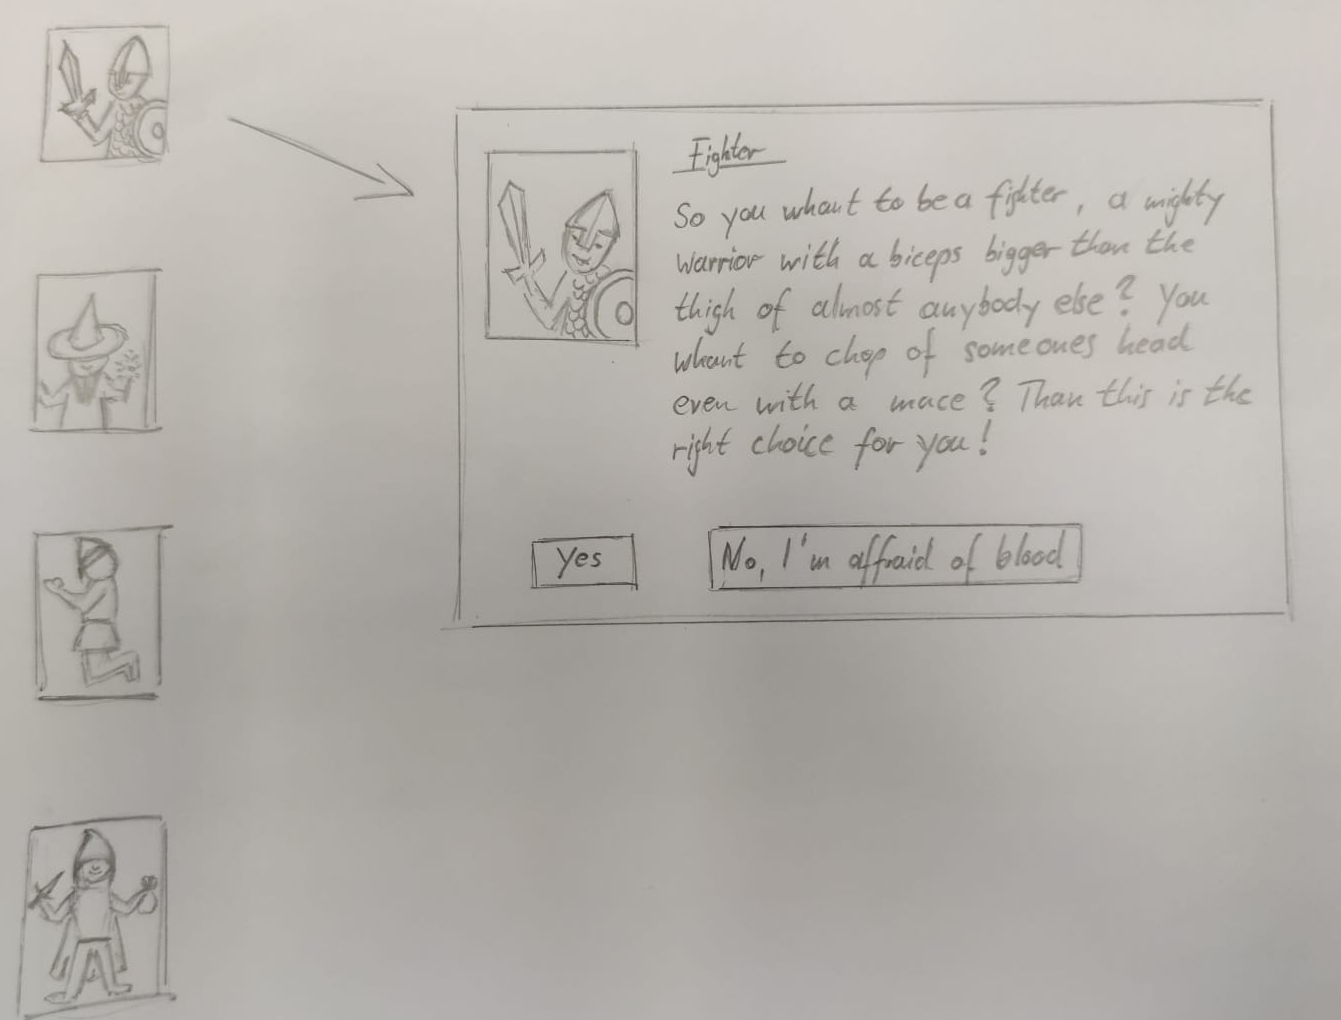
\includegraphics[height=5cm,keepaspectratio]{2021-11-29-Entwurf-Klassen-Ui}
	\\
	Quelle: Homepage von Mark Strehlow, Senior Interaction Designer\\ im Projekt Mira (\href{https://msdo.us/Microsoft-Mira}{msdo.us/Microsoft-Mira})
\end{figure}

Vielmehr sind hier erst noch durch Forschung und Entwicklung für die \ac{WoWi} zu schaffenden und nutzbar zu machenden Geräte gemeint.


\subsection{Gibt es besondere Anforderungen? (technisch, Benutzer, sonstige)}
Beispielinhalt und Texte:

\newpage
\section{Herangehensweise}
Beispielinhalt und Texte:

\subsection{Wie soll das Ziel erreicht werden (Vorgehen, Architektur)}
Beispielinhalt und Texte:

\newpage
\section{Vorstellung des Ergebnisses}
Beispielinhalt und Texte:

\newpage
\section{Reflektion}
Beispielinhalt und Texte:

 die Anwendung wird hier durch eine Betrachtung  der untenstehenden Punkte erfolgen: 
\begin{itemize}
	\item \textbf{Prüfung rechtlicher und IT-technischer Machbarkeit:}
	\\ Neben baurechtlicher Betrachtung hier auch Prüfung in Bezug auf verschiedenartige Realisierungen in Größe, Standort, Bauart und IT-Integration.
	\item \textbf{Aufzeigen und erörtern relevanter Effizienz-Faktoren:}
	\\ Umfasst typisch erwartbare Effizienz-Faktoren wie die Wirtschaftlichkeit ebenso wie auch darüber hinausgehende Auswirkungen die zur ebenso zur Effizienz zu zählen sind.
	\item \textbf{Darstellung möglicher Nutzbarkeiten und Anwendungsfälle:}
	\\ Ausführungen zu erwartbaren Einflüssen auf vorhandene Geschäftsprozesse in der \ac{WoWi} aber auch durch Aufzeigen von neuartigen und darüber hinausgehenden Anwendungsfällen und -bereichen.
\end{itemize}

Diese drei vorgenannten Punkte spiegeln die drei Anforderungen aus der Hypothese der Einleitung wieder und entsprechen dieser genau, in den jeweils genannten Reihenfolgen. 




\end{appendices}
\addtocontents{toc}{\protect\setcounter{tocdepth}{2}}






\newpage % Literaturverzeichnis

% Im Literaturverzeichnis "und" wieder durch "&" ersetzen	
	\DeclareDelimFormat*{finalnamedelim}{\addspace\&\space}

% Punkt hinter und vor der Jahreszahl entfernen	- Wichtig für Quell-Arten wie misc und online -- Sonst ein überflüssiger Punkt im LitVerz.
	\renewbibmacro*{author}{%
	\printtext{%
	\ifnameundef{author}
	{\usebibmacro{labeltitle}}
	{\printnames[apaauthor][-\value{listtotal}]{author}%
	\setunit*{\addspace}%
	\printfield{nameaddon}%
	\ifnameundef{with}
	{}
	{\setunit{}\addspace\mkbibparens{\printtext{\bibstring{with}\addspace}%
	\printnames[apaauthor][-\value{listtotal}]{with}}
	\setunit*{\addspace}}}%
	% \newunit\newblock%
	\usebibmacro{labelyear+extradate}}}

\printbibliography[heading=bibintoc,title=Literaturverzeichnis]

\newpage % Ehrenwörtliche Erklärung
\pagenumbering{gobble} % Keine Seitenzahlen mehr
\section*{Ehrenwörtliche Erklärung} 
	Hiermit versichere ich, dass die vorliegende Arbeit von mir selbstständig und ohne unerlaubte Hilfe angefertigt worden ist, insbesondere dass ich alle Stellen, die wörtlich oder annähernd wörtlich aus Veröffentlichungen entnommen sind, durch Zitate als solche gekennzeichnet habe. Weiterhin erkläre ich, dass die Arbeit in gleicher oder ähnlicher Form noch keiner Prüfungsbehörde/Prüfungsstelle vorgelegen hat. Ich erkläre mich damit \textbf{nicht einverstanden}, dass die Arbeit der Öffentlichkeit zugänglich gemacht wird. Ich erkläre mich damit einverstanden, dass die Digitalversion dieser Arbeit zwecks Plagiatsprüfung auf die Server externer Anbieter hochgeladen werden darf. Die Plagiatsprüfung stellt keine Zurverfügungstellung für die Öffentlichkeit dar.

			\par\medskip
			\par\medskip

			\vspace{5cm}

			\begin{table}[H]
				\centering
				\begin{tabular*}{\textwidth}{c @{\extracolsep{\fill}} ccccc}
					
					\myOrt, \the\day.\the\month.\the\year
					&
					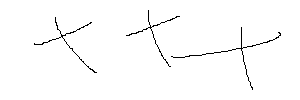
\includegraphics[width=0.35\textwidth]{unterschrift_rico}\vspace*{-0.35cm}
					\\
					\rule[0.5ex]{12em}{0.55pt} & \rule[0.5ex]{12em}{0.55pt} \\
					(Ort, Datum) & (Rico ) 
					\\

					
					  
					&
					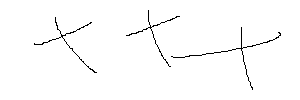
\includegraphics[width=0.35\textwidth]{unterschrift_henning}\vspace*{-0.35cm}
					\\
					 & \rule[0.5ex]{12em}{0.55pt} \\
					& (Henning ) 
					\\

					
					  
					&
					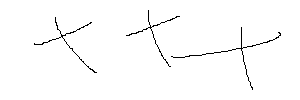
\includegraphics[width=0.35\textwidth]{unterschrift_julian.png}\vspace*{-0.35cm}
					\\
					 & \rule[0.5ex]{12em}{0.55pt} \\
					 & (Julian ) 
					\\



				\end{tabular*} \\
			\end{table}

\end{document}